\chapter{Interpretation for Resonance Analysis}
\chapterquote{The best things happen by chance.}{Dory, Finding Dory}
\label{Ch:resonance_stat}
After obtaining the $m_{WV}$ distributions from both control and signal regions, a statistical interpretation is used to determine whether any signal signature is captured in this analysis. The statistical analysis uses the following steps:

\begin{itemize}
	\item{Variation on Histograms}: Systematic uncertainties are applied in the analysis to vary the variables like the jet energy or event weight on the simulation samples. This then leads to the variations on distribution of $m_WV$, and each systematic uncertainty gives one varied $m_{WV}$ histogram. Those histograms are then taken into the statistic interpretation with the one without any variation (this is called ``nominal'' histogram) for following steps. 

	\item{Simultaneous Fitting}: a binned maximum-likelihood fitting is performed in control and signal region histograms simultaneously to rescale the backgrounds and signal for a proper agreement to the data. The scaling is performed bin-by-bin in histograms of $m_{WV}$ distribution, which means the shape of $m_{WV}$ distribution would change under this step. Further detail will be discussed later.
	
	\item{Signal Verification}: the signal interpretation is through the CLs method by quantifying the agreement between data and background in signal regions after simultaneous fitting. The result will be presented as the exclusion on the mass regions at $95\%$ confidence level or the discovery with a corresponding ``p-value''.
\end{itemize}
The details of each step will be discussed in the following sections with the results from this analysis, and the details of the methodology formalism can be referred to \cite{StatisticsData}.
\section{Systematic Uncertainties}
No measurement and theoretical estimation could be $100\%$ accurate, and the uncertainties would propagate to the $m_{WV}$ histograms. In this case, a bump in data might be due to the uncertainty fluctuation but mistaken as a signal. To prevent such a mistake, both systematic and statistic uncertainties are brought into the consideration for the ground fitting and signal interpretation. The following are the systematic uncertainties considered in this analysis and how they are taken into the $m_{WV}$ histograms, and the methods to estimate the uncertainties of each source could be found in \cite{PERF-2016-01,ATL-PHYS-PUB-2015-037,ATLAS:2019pzw,PERF-2016-04,ATLAS-CONF-2014-018,Herde:2059849}.
\begin{itemize}
	\item{\bf Luminosity Measurement}: the given luminosity of the dataset collected in 2015 and 2016 is accompanied by the uncertainty of $2.1\%$. It is applied in the histograms from simulations by scaling up and down the total yield of each bin by $2.1\%$.

	\item{\bf Selection and Reconstruction Efficiency}: the object reconstruction and selection efficiency of physical objects are not consistent between data and simulation like the trigger efficiency shown in Subsec.~\ref{Subsec:Trigger_resonance}. This type of uncertainties are induced by the uncertainties in variables used in tag and probe method. To estimate the impact, the tag and probe criteria are tightened and loosened for scale factor re-estimation, and they replace the nominal scale factors to obtain the new histograms. This type of uncertainties come from the efficiencies of trigger, lepton isolation, lepton identification, jet b-tagging, fat jet boson-tagging, and all physical object reconstruction, and each of them gives one uncertainty contribution with a pair of histograms. (loosened and tightened criteria give two histograms for each source.)

	\item{\bf Energy Scale and Resolution}: the energy measurement is based on the pulse shapes from the calorimeter cells, but it is not precise enough due to different responses of layers or varied granularities of the calorimeter. The uncertainty estimation of this source for electrons and muons are via the $Z$ boson mass reconstruction in dedicated analysis as a function of $p_{T}$. In the case of jets, they are estimated via the comparison of the MC truth and reconstructed $E_{T}$ from dijet simulation samples with the variation on multiple sources, which contributes 81 uncertainties. However, a simplified scheme is applied to combine related uncertainties into 21 categories, for which details could be found in \cite{Herde:2059849}. The measurement uncertainties of jets also have impact on $E^{miss}_{T}$ reconstruction, and the variation on jet energy scale is the dominant contribution to $E^{miss}_{T}$ uncertainty. Each variation is applied on the corresponding object $E_{T}$, which gives varied $m_{WV}$ histograms of dedicated uncertainty contributions.

	\item{\bf Simulation Modelling}: The tuning and modelling parameters are different for generators and showering models due to the varied preference of theoretical approximation. To take this variation into the uncertainty contribution, simulated samples are regenerated with another simulation sets (a different generator or tuning parameters), and the same events selections is applied. New histograms are then obtained after the normalization to total event yield of the nominal sample after the simultaneous fitting (the explanation is in the next section). Each tuning of one SM background process or signal sample gives one uncertainty contribution. For W+jet and $t\bar{t}$ backgrounds, the varied histograms are not taken into the simultaneous fitting directly due to the poor statistics in the region of high $m_{WV}$. A linear fitting in the dedicated control regions is performed to smooth the $m_{WV}$ distribution based on the event ratio between nominal and varied histograms respectively for each category and each background (the linear fitting of W+jet ($t\bar{t}$) is performed in the W+jet ($t\bar{t}$) control region), which gives weights as a function of $m_{WV}$ in the following form:
	\begin{equation}
	w = a + b\times m_{WV}
	\end{equation}
	with a and b as fitting parameters, and w as the given scale factor for each bin to modify the $m_{WV}$ distribution. The rescaled histograms are then taken into the next step for simultaneous fitting. For the signal modelling uncertainty, the generator tuning is to consider additional jets from the initial and final state radiations (ISR and FSR), and histograms from the new tunings are taken into next step without the process done for W+jet and $t\bar{t}$ modelling uncertainties. For other minor SM background contributions, this uncertainty is taken negligible.
	\item{\bf Multijet Background Modelling}: multijet modelling is sensitive to the lepton isolation criteria and the jet topology. To estimate the uncertainty of this contribution, the fake factors were re-evaluated with loosened and tightened isolations on leptons as well as in the single b-jet control region, and the new fake factors are applied to get the new multijet $m_{WV}$ distribution.
\end{itemize}
\section{Likelihood Construction $\&$ Fitting}
A binned simultaneous fit is conducted to adjust the background and signal to agree well with the data in the $m_{WV}$ distribution. The following is the binning used for boosted (ranged from 500~GeV to 6~TeV, Eq.~\ref{Eq:boosted_mbin}) and resolved (ranged from 300~TeV to 2~TeV, Eq.~\ref{Eq:resolved_mbin}) category histograms:

\begin{multline}
\label{Eq:boosted_mbin}
m^{Boosted}_{WV}= [500, 575, 660, 755, 860, 975, 1100, 1235, 1380, 1535, 1700,\\ 1875, 2060, 2255, 2460, 2675, 2900, 3135, 3380, 3800, 6000]
\end{multline}
\noindent
\begin{equation}
\label{Eq:resolved_mbin}
m^{Resolved}_{WV}= [300, 360, 420, 500, 575, 660, 755, 860, 975, 1100, 1500, 2000]
\end{equation}
\noindent
For the VBF category, the bins with higher $m_{WV}$ have the statistics too low for the MC samples, so there is only one bin  for  $m_{WV}>1535~GeV$($1100~GeV$) for the boosted (resolved) region. Then, a maximum likelihood method is performed for the fitting which could be presented in the full form as:
\begin{align}
\label{Eq. ML_all}
 \mathcal{L}(\mu, \mbox{\boldmath $\theta$}) = \displaystyle\prod_{k} \left\{
 \displaystyle\prod_{i=1}^{N_{\rm bins}^{k}}\left[
       P(N_{i}^{k}|\mu s_{i}^{k} + \mu_{t\bar{t},k} b_{t\bar{t},i}^{k} + \mu_{W,k} b_{W,i}^{k} + b_{{\rm others},i}^{k})
       \times\displaystyle\prod_{j=1}^{N_{\theta}}{\rm Nuis}(\theta_0|\theta_{j,k})
       \right]
 \right\} %\nonumber \\
% \displaystyle\prod_{l=1}^{N_{{\rm bins},k}^{TR}}P(N_{kl}^{TR}|\mu s_{kl}^{TR} + \mu_{t\bar{t},k} b_{t\bar{t},kl}^{TR} + \mu_{W,k} b_{W,kl}^{TR} + b_{{\rm others},m}^{TR})
% \times \nonumber \\
% \left. \displaystyle\prod_{m=1}^{N_{{\rm bins},k}^{WR}}P(N_{km}^{WR}|\mu s_{km}^{WR} + \mu_{t\bar{t},k} b_{t\bar{t},km}^{WR} + \mu_{W,k} b_{W,km}^{WR} + b_{{\rm others},m}^{WR})
% \right\} \nonumber \\
% \times\displaystyle\prod_{j=1}^{N_{\theta}}{\rm Nuis}(\theta_j)
\end{align}
where $P(x|y)$ is the Poisson probability distribution function (p.d.f.) to observe ``x'' number of events (data) when ``y'' number of events are expected from theory (estimated event number sum of signal event number, s, and background event number, b) in each bin which is indexed by $i$. To properly normalize the background, $\mu$'s are the most important parameter in the formula as floating parameters to rescale the event numbers in each region for background estimation , and they are shared between control and signal regions (simultaneously). The $\mu$ to rescale the signal event number is also called ``signal strength'' which is the primary parameter of interest in the statistical interpretation. The k index in this formula corresponds to the event categories of each control/signal region: ggF merged HP, ggF merged LP, ggF resolved, VBF merged HP, VBF merged LP, and VBF resolved regions for W+jet control regions, $t\bar{t}$ control regions and signal regions. For the last term, ${N_{\theta}}{\rm Nuis}(\theta_0|\theta_j)$, it is to take systematic uncertainties into the likelihood as nuisance parameters to further vary the probability distribution, which will be discussed next. 
\\
\\{\bf Nuisance Parameters}
\\
\\The last term in Eq. \ref{Eq. ML_all} is to take in the consideration of systematic uncertainties mentioned in the last section. They are called ``nuisance parameters''  (NP) in the scope of statistics, as they are of the second interest with respect to the primary parameter of interest (POI), $\mu$, the scale factor for signal events. Nuisance parameters are used as addition probabilities multiplying the Poisson distribution function which could be seen in one bin as:
\begin{equation}
p = P(x|\mu n_0)\times\displaystyle\prod_{j=1}^{N_{\theta}}{\rm Nuis}(\theta_0|\theta_j)
\end{equation}
Under this equation, $P(x|\mu n_0)$ is a simplified form of Eq.~\ref{Eq. ML_all}, and the nuisance parameter form is taken as the probability to have $\theta_j$ variation with respect to an nominal value, $\theta_0$ (j is the index for NPs).
\\
\\There are three types of nuisance parameters based on their impact on the distribution of $m_{WV}$ \cite{NuiTreats}. The following are the treatments to them in this analysis, and most of them are taking the constraint as a Gaussian distribution, although the other p.d.f. options are also available. (In the following content, the NP contribution to the likelihood is not normalized to 1, because the normalization factors are cancelled out in the form of a ratio in the next step.)
\begin{itemize}
	\item Statistical Uncertainty: with the limited event numbers of background estimation, the statistical uncertainties are taken as extra nuisance parameters. A light Beeston-Barlow method is applied which introduces a new scale factor, $\theta$, on each bin with the constraint of a Gaussian distribution with the default value as 1. These nuisance parameters are then contributed to the likelihood in this expression:
	\begin{equation}
	Nuis(1|\theta) = \exp{\left[\frac{(\theta-1)^2}{2\sigma^{2}}\right]}
	\end{equation} 
	$\theta$ is the ratio of the scaled event number to the unscaled (raw) event number in the prediction in one bin with i as the bin index, and the distribution width, $\sigma$ is computed as the quadratic sum of all the background contributions. Each bin in the histograms makes one contribution in the likelihood with this formulation.
 
	\item Overall Normalization: this type of nuisance parameters arise, when yields of $m_{WV}$ histograms are scaled up and down without changing the shape of distributions. They are contributed by uncertainties from the scaling factors and luminosity measurement. The treatment is simply taking a Gaussian distribution for the related probability. It can be presented in the likelihood as:
	\begin{equation}
	Nuis(N|\theta)=\exp\left[\frac{(\theta-N)^2}{2\sigma^2}\right]
	\end{equation}
	In this expression, the Gaussian distribution has the mean of estimated event number, N, with the width of observed uncertainty, $\sigma$. For the case of luminosity, $\sigma$ is taken as $2.1\%$ of the estimated event number. In the case of uncertainties for scale factors, Tab. \ref{Tab:constaints} is the summary for $\sigma$ applied on different background scale factors. For $t\bar{t}$ and W+jets backgrounds, no constraint is set, and the deviation of $\theta$ from N for their scale factors is always taken as 1$\sigma$.  
	
	\begin{table}[h]
		\caption{The constraints on scaling factors for SM backgrounds}
		\renewcommand{\arraystretch}{1.3}
		\centering
		\begin{tabular}{| c | c | c |  }
			\hline
			\hline
			Background      &     Constraint     & Uncertainty ($\sigma$)   \\
			\hline
			W+jets          &     Free           & 1                          \\
			\hline
			$t\bar{t}$      &     Free           & 1                          \\
			\hline
			single top      &     Gaussian       & 0.11                        \\
			\hline
			WW+WZ           &     Gaussian       & 0.3                         \\
			\hline
			Z+jets          &     Gaussian       & 0.11                        \\
			\hline
		\end{tabular}
	\label{Tab:constaints}
    \end{table}

	\item Shape Related Uncertainty: for the uncertainties which are asymmetrically sided ($\sigma_{+}\neq\sigma_{-}$, $\sigma_+$ and $\sigma_-$ are event numbers in the varied histograms for a given systematic uncertainty), a procedure called ``morphing'' is applied on each bin respectively which could be presented as:
    \begin{equation}
    n =
    \begin{cases}
    n_0+ \theta(\sigma_{+}-n_0) & \theta>0 \\
    n_0+ \theta(n_0-\sigma_{-}) & \theta<0
    \end{cases}
    \end{equation}
    Here, $n$ is the scaled event number, while $n_0$ is the raw event number. Then, scaled factor is constrained by $\theta$ which is under a Gaussian distribution constraint ($G(\mu, \sigma)=G(0,1)$). This type of nuisance parameters cover the most of systematic uncertainties like selection and reconstruction efficiencies, energy scale, or theoretical modelling. 
\end{itemize}
\noindent
{\bf Quality of Fitting}
\\
\\To find the maximum of likelihood in Eq. \ref{Eq. ML_all}, the logarithmic form, $\log{\mathcal{L}}$, is used. The extreme value is then found when:
\begin{equation}
-\frac{\partial}{\partial\mu}\log{\mathcal{L}} = 0
\end{equation}
However, the phase space of the likelihood is complex constructed with multiple dimensions of the scale factors, so the MINUIT2\cite{minuit} method with Hessian matrix\footnote{Hessian matrix is a square matrix of second-order partial derivatives of a scalar-valued(i.e. the likelihood) function} is performed under the framework of RooStat\cite{Moneta:2010pm}. The maximized likelihood is denoted as: $\mathcal{L}(\hat{\mu}, \hat{\theta})$
\\
\\To verify the quality of the process of fitting with the likelihood equation, two properties of the results are verified: 
\begin{itemize}
	\item {\bf Pull} The pull is defined as the deviation of nuisance parameters from the expected mean number:
	\begin{equation}
	pull=\frac{\hat{\theta}-\theta_0}{\sigma_{\theta}}
	\end{equation}
	with $\theta_0$ as the mean of $\theta$, while the uncertainty of nuisance parameters, $\sigma_\theta$, is taken from the likelihood phase space. The pull result is verified by the comparison to ``Asimov data'' which took the expected event number as the observed data. (so the Asimov data has the pull as 0.)  The proper fitting should have all the pulls within the $1\sigma$ variation with the reasonable uncertainty, or that indicates a huge discrepancy between the background estimation and the observed data. 
	\item {\bf Nuisance Parameter Correlation} The phase space of likelihood is constructed under the assumption that all the nuisance parameters are uncorrelated, but it still needs to be verified. The correlation matrix is then used for this verification which has the elements defined as:
	\begin{equation}
	Cov(\theta_i, \theta_j) = \frac{\partial^2\log(\mathcal{L})}{\partial\theta_i \partial\theta_j}|_{\theta=\hat{\theta}}
	\end{equation}
	This element, $Cov(\theta_i, \theta_j)$, should be close to 0 if $i\neq j$.
\end{itemize}
The pulls are with the signal of ggF 2000$~GeV$ and 500$~GeV$ W' bosons for boosted and resolved categories which are presented in Fig. \ref{Fig:pull_HVT} with signal strength (signal scale factor) as 0\footnote{The signal sample was used as an essential element for the statistics tool configuration, but the choice does not affect the result}. Fig. \ref{Fig:Cor_HVT} is the correlation matrix of the nuisance parameters applied in the ggF HP boosted region. The normalization factors could be seen over-constrained and over-pulled in the fitting, as the scaling factors are allowed to be pulled to the extreme for better data-background agreement after the fitting \cite{EXOT-2016-28}. And, it could also be observed that the resolved channel has the NPs pulled and constrained much more than the merged channel, and this is due to the fact that the $m_{WV}$ shape was significantly affected by the systematic uncertainty variations in the resolved event categories, and this could also be seen in Tab. \ref{Tab:lvqq_fittedsf} that the scale factors in the resolved regions have larger deviation from one with respect to the two merged regions. The final yields for the background only fitting are then shown in Tab.~\ref{tab:yields_WW} (WW) and Tab.~\ref{tab:yields_WZ} (WZ) for the ggF/DY event category, and the VBF ones are shown in Tab.~\ref{tab:yields_VBFWW} (WW) and Tab.~\ref{tab:yields_VBFWZ} (WZ). It could be noted that the total uncertainties in event yields are smaller than the ones shown in Sec.~\ref{Sec:data_bkg_compar}. The difference here is that the uncertainties in Sec.~\ref{Sec:data_bkg_compar} was derived as the quadratic sum over all the uncertainties, but the ones presented in the yields tables are the uncertainties along the statistical uncertainty in the phases space of the likelihood.  
\begin{figure}[!h]                
	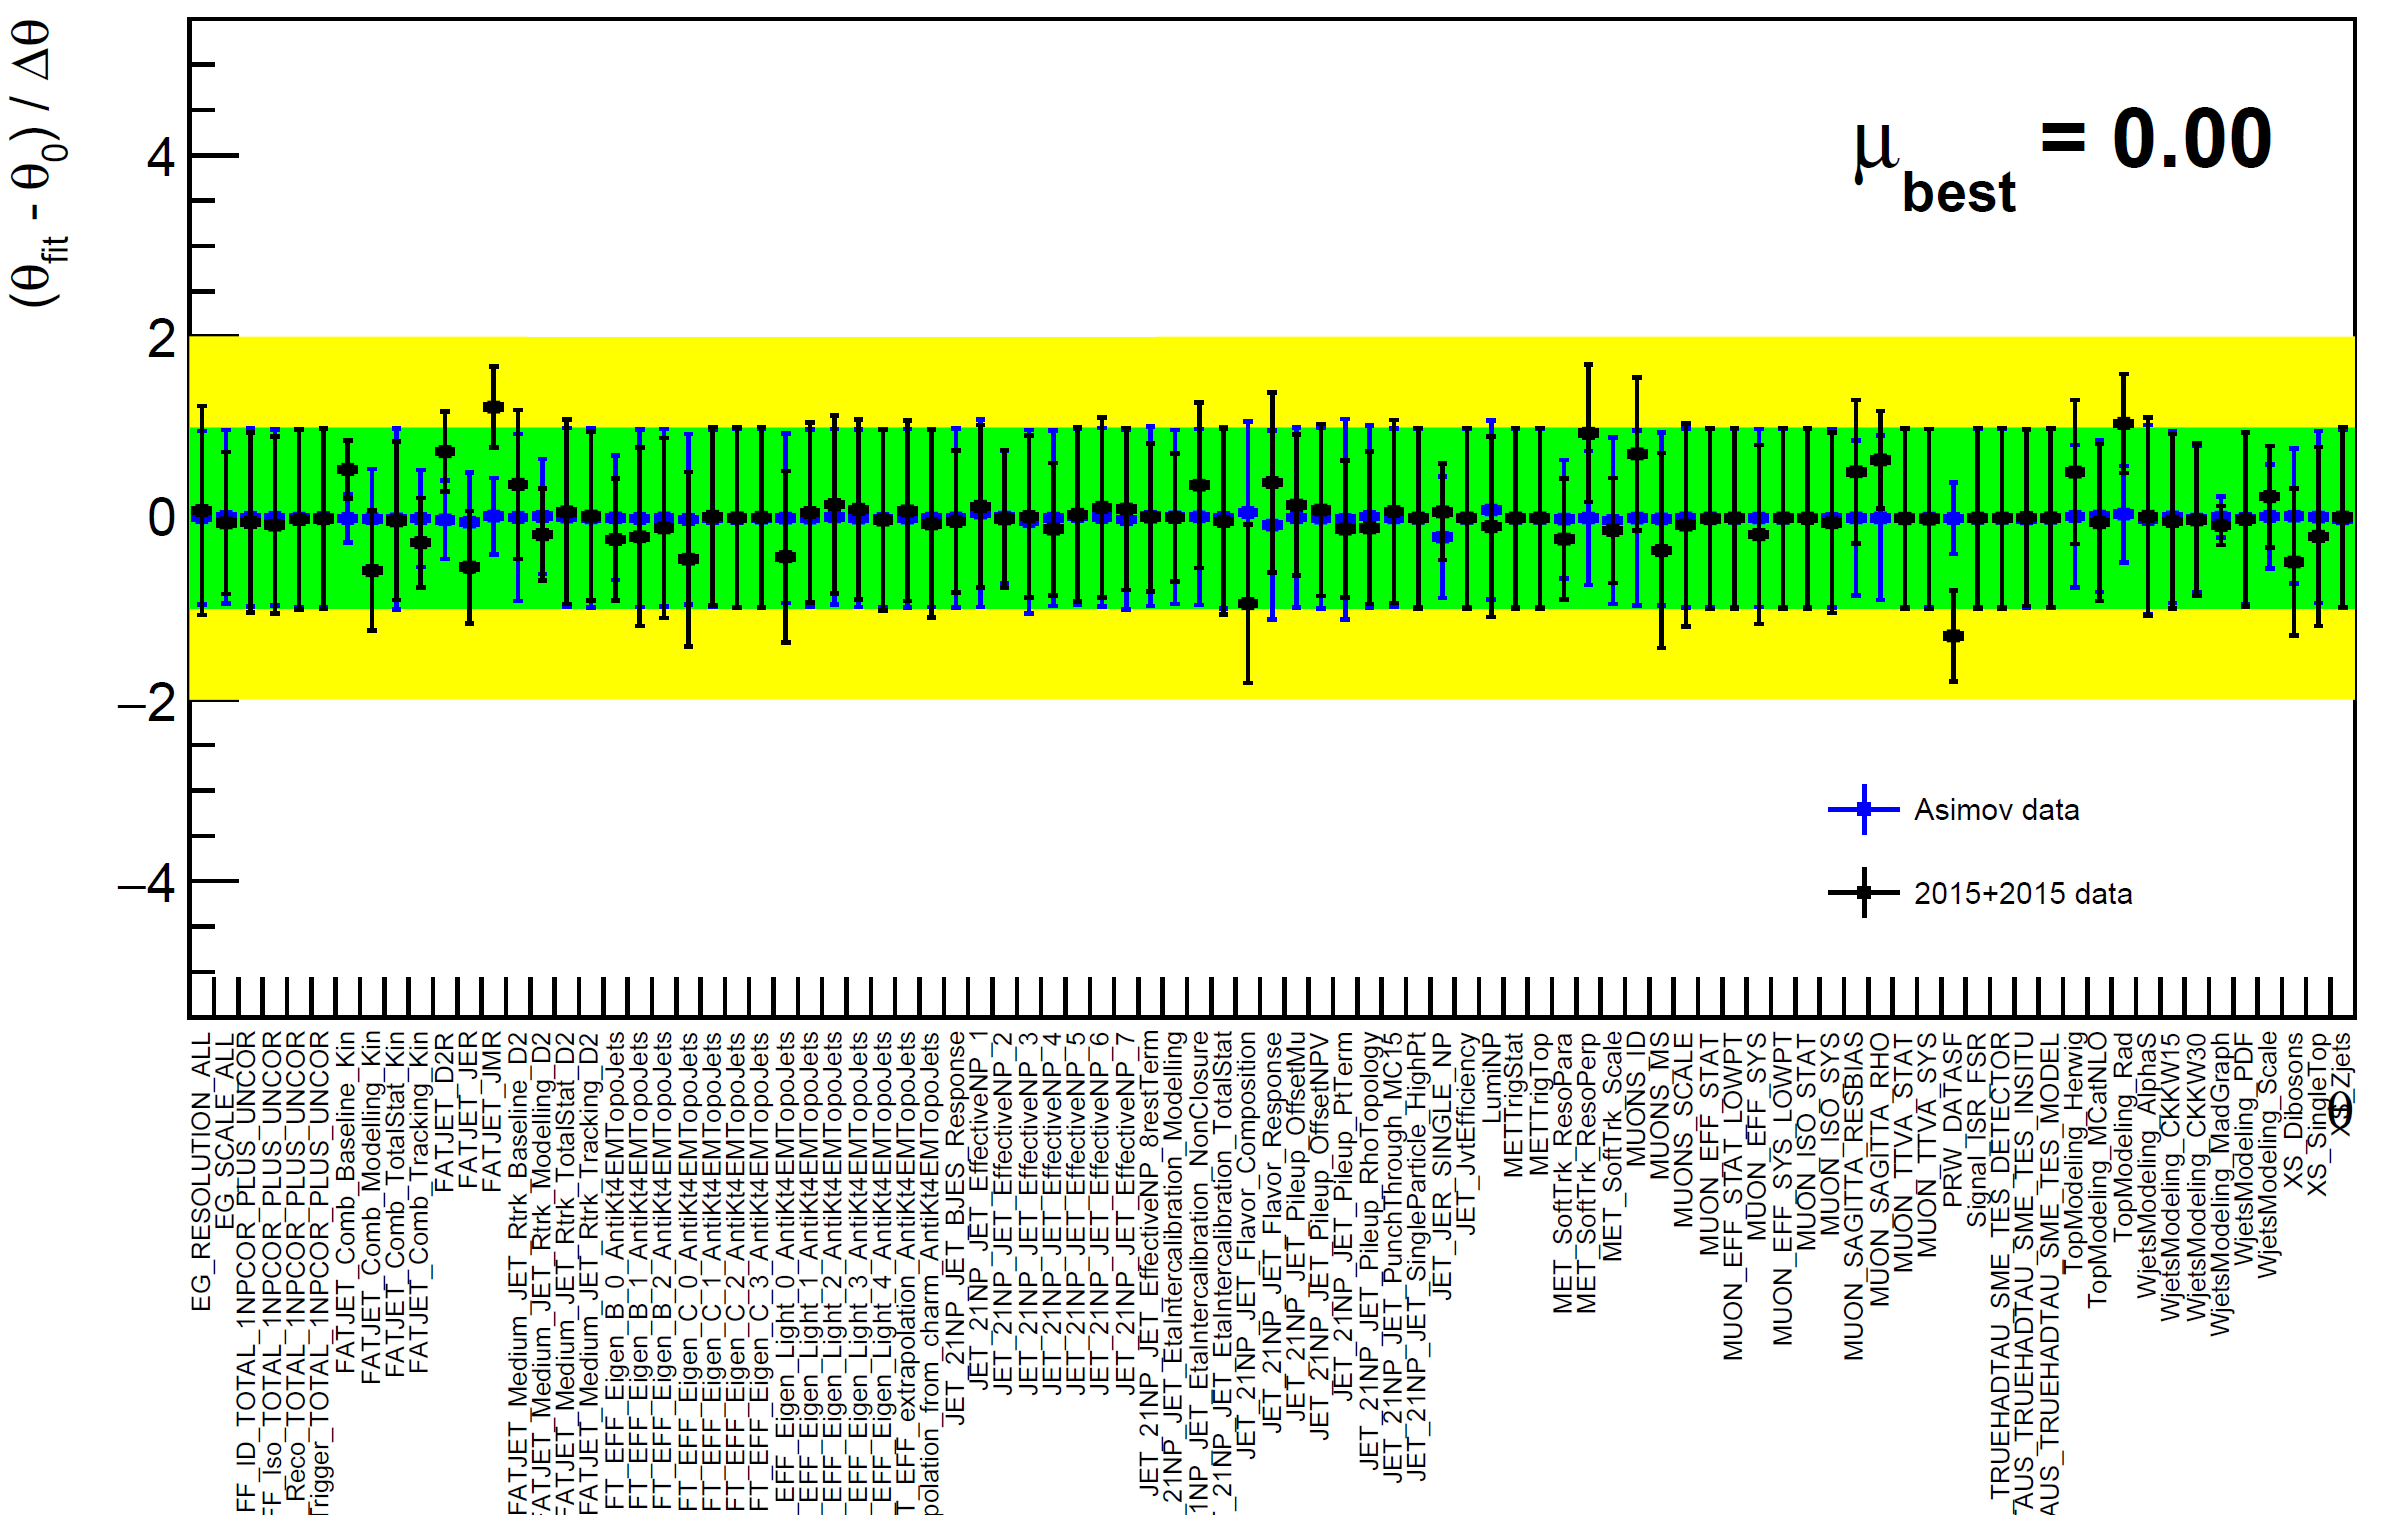
\includegraphics[width=0.81\textwidth]{Chapter4/NuiPull_ggFHVT2000.png}
	 \vspace{5mm}
	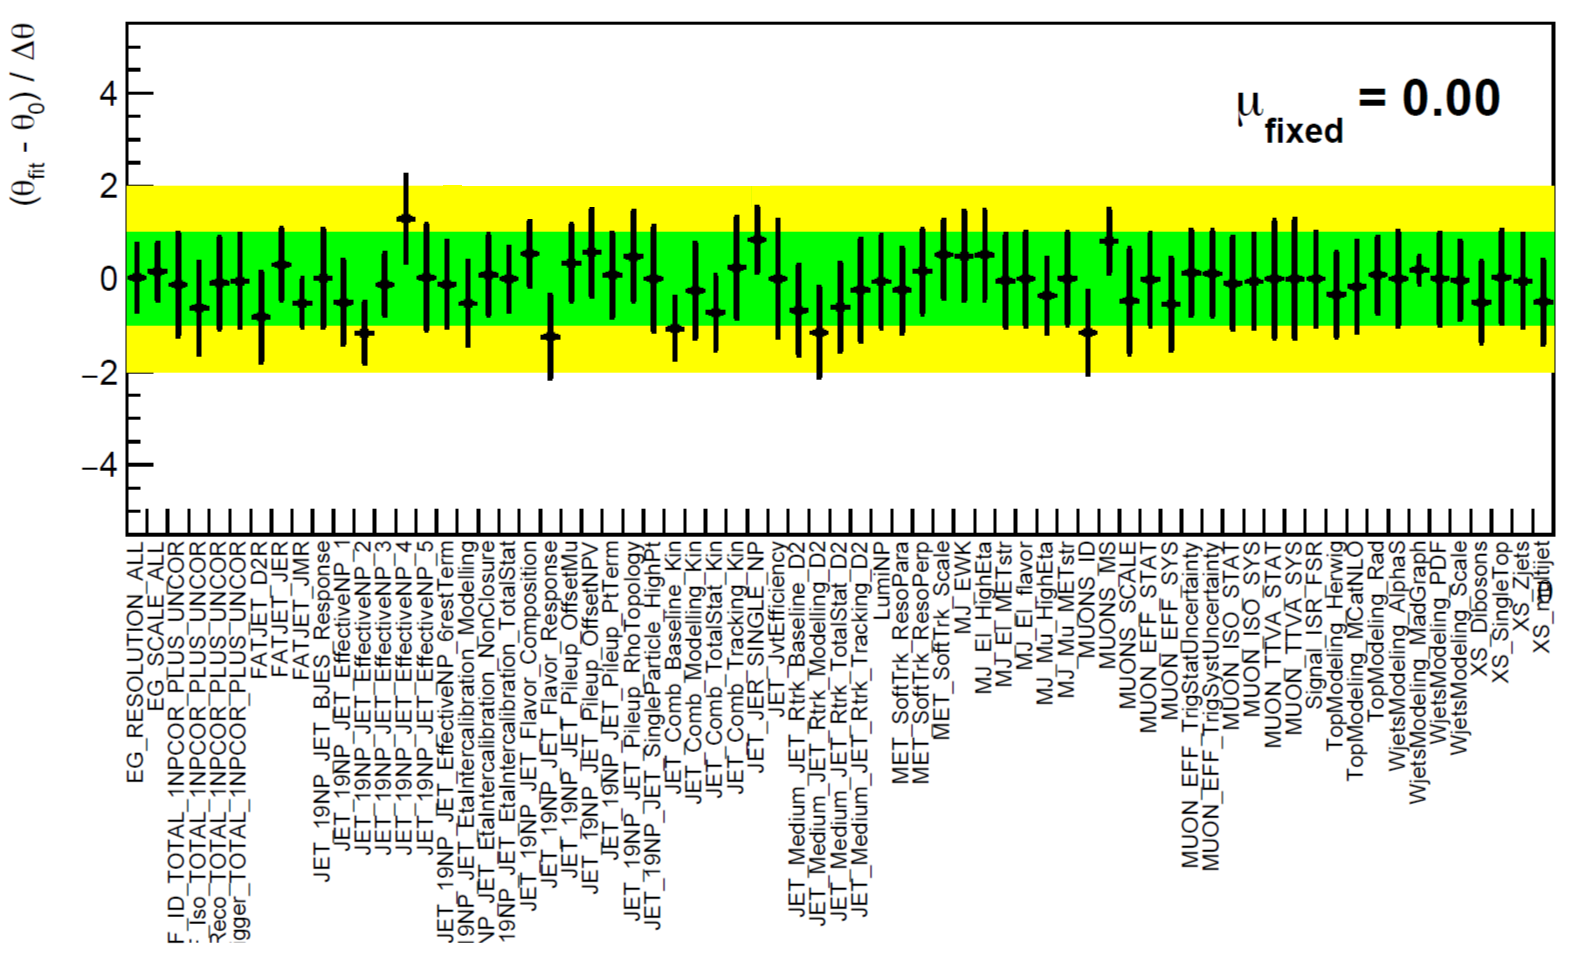
\includegraphics[width=0.81\textwidth]{Chapter4/NuiPull_ggFHVT500.png}
	\centering
	\begin{center}
		\caption{The pulls for the fitting with input signal of ggF 2$~TeV$ (up) and  500$~GeV$ (down) W' bosons for the boosted and resolved categories respectively.}
		\label{Fig:pull_HVT}            
	\end{center}
\end{figure} 
\begin{figure}[!h]
	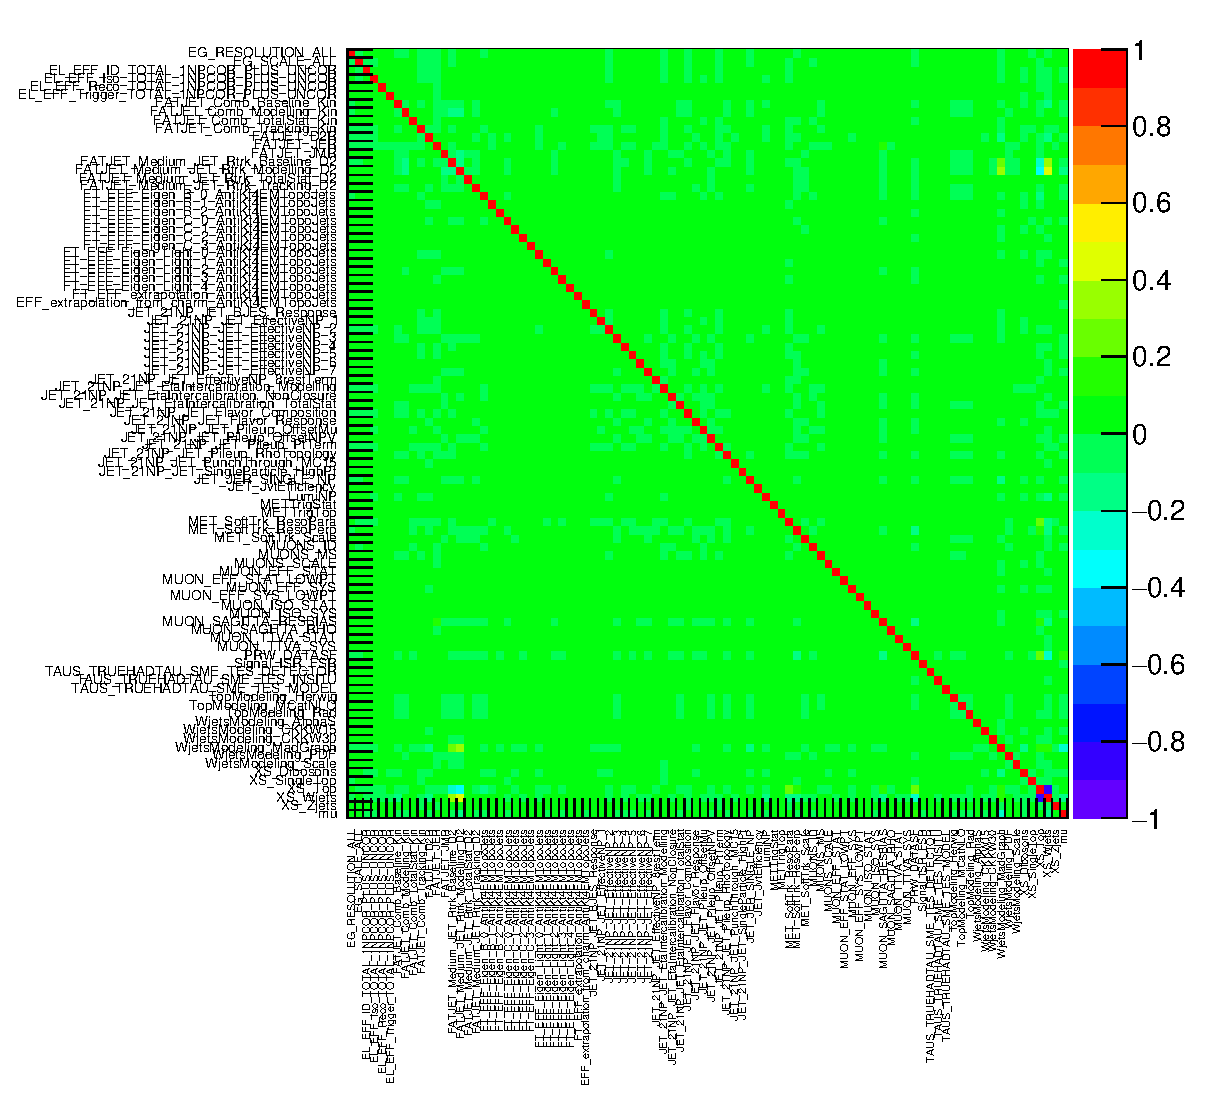
\includegraphics[width=1.0\textwidth]{Chapter4/CorrMatrix_WW_HP_ggF.eps}
	\begin{center}
		\caption{The correlation matrix of boosted high purity region with the ggF event selection}
		\label{Fig:Cor_HVT}
	\end{center}
\end{figure}
\begin{table}
   \begin{center}
   	\resizebox{\textwidth}{!}{
   		 \begin{tabular}{|l|c|c|c|c|c|}
   		 	\hline
   		 	\multicolumn{2}{|l|}{\multirow{2}{*}{Control regions}} & \multicolumn{2}{c|}{WW}  &  \multicolumn{2}{c|}{WZ} \\
   		 	\cline{3-6}
   		 	\multicolumn{2}{|l|}{} & ggF & VBF & ggF & VBF \\
   		 	\hline
   		 	\multirow{3}{*}{W+jet CR} & Merged HP & $0.94\pm0.07$ & $0.87\pm0.29$ & $0.95\pm0.07$&$0.85\pm0.28$ \\
   		 	\cline{2-6}
   		 	                          & Merged LP & $0.97\pm0.07$ & $0.86\pm0.23$ & $0.98\pm0.07$&$0.86\pm0.22$ \\
   		 	\cline{2-6}
   		 	                          & resolved  & $0.87\pm 0.08$ & N/A & $0.90\pm0.08$& $0.68\pm0.23$ \\
   		 	\hline
   		    \multirow{3}{*}{$t\bar{t}$ CR} & Merged HP & $0.92\pm0.07$ & $1.16\pm0.27$ & $0.93\pm0.08$&$1.03\pm0.21$ \\
   		 	\cline{2-6}
                                      & Merged LP & $0.97\pm0.07$ & $1.21\pm0.28$ & $0.96\pm0.07$&$1.12\pm0.24$ \\
   		 	\cline{2-6}
                                      & resolved  & $0.90\pm 0.07$ & N/A & $0.92\pm0.06$& $1.03\pm0.27$\\
            \hline
   		 	
   		 \end{tabular}
   }
   \caption{The scale factors for the W+jet ($\mu_w$) and $t\bar{t}$ ($\mu_{t\bar{t}}$) backgrounds for the fitting with the signal strength, $\mu$, set at 0}
   \label{Tab:lvqq_fittedsf}
   \end{center}
\end{table}

\begin{table}[tbp]
	\renewcommand{\arraystretch}{1.25}
	\caption{Expected and observed yields in signal and control regions for the ggF/DY $WW$ signal hypothesis.  Yields and uncertainties are evaluated after a background-only fit to the data in all regions indicated above.}
	\begin{center}
		\resizebox{\textwidth}{!}{%
			\begin{tabular}{| c | c@{\ $\pm$\ }c c@{\ $\pm$\ }c c@{\ $\pm$\ }c | c@{\ $\pm$\ }c  c@{\ $\pm$\ }c c@{\ $\pm$\ }c | c@{\ $\pm$\ }c  c@{\ $\pm$\ }c c@{\ $\pm$\ }c |}
				\hline
				\hline
				&\multicolumn{6}{c|}{Boosted, High Purity}  &\multicolumn{6}{c|}{Boosted, Low Purity}  &\multicolumn{6}{c|}{Resolved}   \\
				\cline{1-19}
				&\multicolumn{2}{c}{               SR}&\multicolumn{2}{c}{      $W$+jets CR}&\multicolumn{2}{c|}{           Top CR}&\multicolumn{2}{c}{    Signal Region}&\multicolumn{2}{c}{      $W$+jets CR}&\multicolumn{2}{c|}{           Top CR}&\multicolumn{2}{c}{               SR}&\multicolumn{2}{c}{      $W$+jets CR}&\multicolumn{2}{c|}{           Top CR}\\
				\hline
				$W$+jets    & 3116&165 & 6848&206 &  540&60  & 10790&251 & 10972&255 & 1424&167 & 61537&1826 & 165656&722  &  7951&925   \\
				$t\bar{t}$  & 2043&142 & 2920&180 & 6883&138 &  2648&187 &  3790&222 & 8738&235 & 23287&1633 &  31110&2050 & 78354&1262  \\
				Single-$t$  &  374&44  &  487&57  &  704&84  &   493&56  &   553&64  &  819&97  &  3822&436  &   4675&539  &  5631&669   \\
				SM Diboson  &  353&94  &  167&45  &   51&14  &   431&118 &   201&55  &   70&20  &  2413&656  &   1500&408  &   274&77    \\
				$Z$+jets    &   49&6   &  143&17  &   15&3   &   205&25  &   215&27  &   54&9   &  1748&273  &   4298&640  &   275&62    \\
				Multijet    &\multicolumn{2}{c}{--}&\multicolumn{2}{c}{--}&\multicolumn{2}{c|}{--}&\multicolumn{2}{c}{--}&\multicolumn{2}{c}{--}&\multicolumn{2}{c|}{--}& 
				                3601&720 & 7627& 1671& 799&137\\
				\hline
				Total&        5935&70  &10565&96  & 8192&87  & 14566&120 & 15730&124 & 11105&104& 96409&310  & 214866&468  & 93283&307   \\
				\hline
				Observed&\multicolumn{2}{c}{5885}             &\multicolumn{2}{c}{10619}             &\multicolumn{2}{c|}{8178}             &\multicolumn{2}{c}{14566}             &\multicolumn{2}{c}{15707}             &\multicolumn{2}{c|}{11133}             &\multicolumn{2}{c}{96459}             &\multicolumn{2}{c}{214838}             &\multicolumn{2}{c|}{93257}             \\
				\hline
				\hline
			\end{tabular}
		}
		\label{tab:yields_WW}
	\end{center}
\end{table}



\begin{table}[tbp]
	\renewcommand{\arraystretch}{1.25}
	\caption{Expected and observed yields in signal and control regions for the $WZ$ signal hypothesis.  Yields and uncertainties are evaluated after a background-only fit to the data in all regions indicated above.}
	\begin{center}
		\resizebox{\textwidth}{!}{%
			\begin{tabular}{| c | c@{\ $\pm$\ }c c@{\ $\pm$\ }c c@{\ $\pm$\ }c | c@{\ $\pm$\ }c  c@{\ $\pm$\ }c c@{\ $\pm$\ }c | c@{\ $\pm$\ }c  c@{\ $\pm$\ }c c@{\ $\pm$\ }c |}
				\hline
				\hline
				&\multicolumn{6}{c|}{Boosted, High Purity}  &\multicolumn{6}{c|}{Boosted, Low Purity}  &\multicolumn{6}{c|}{Resolved}   \\
				\cline{1-19}
				&\multicolumn{2}{c}{               SR}&\multicolumn{2}{c}{      $W$+jets CR}&\multicolumn{2}{c|}{           Top CR}&\multicolumn{2}{c}{    Signal Region}&\multicolumn{2}{c}{      $W$+jets CR}&\multicolumn{2}{c|}{           Top CR}&\multicolumn{2}{c}{               SR}&\multicolumn{2}{c}{      $W$+jets CR}&\multicolumn{2}{c|}{           Top CR}\\
				\hline
				$W$+jets&                   3679 &         173&                   6958 &         191&                    556 &          61&                  13356 &         299&                  11091 &         247&                   1496 &         173&                  49052 &        1294&                 164656 &        2692&                   8066 &         921\\
				$t\bar{t}$&                   2283 &         146&                   2812 &         167&                   6842 &         141&                   3447 &         233&                   3681 &         218&                   8611 &         241&                  24376 &        1272&                  30589 &        1955&                  78012 &        1269\\
				Single-$t$&                    410 &          50&                    485 &          57&                    749 &          90&                    655 &          75&                    556 &          65&                    854 &         102&                   3499 &         399&                   4743 &         549&                   5762 &         685\\
				SM Diboson&                    356 &          98&                    162 &          44&                     51 &          14&                    498 &         138&                    193 &          53&                     71 &          21&                   1672 &         470&                   1466 &         404&                    267 &          78\\
				$Z$+jets&                     56 &           7&                    148 &          18&                     15 &           3&                    244 &          31&                    212 &          26&                     55 &           9&                   1475 &         259&                   4406 &         659&                    282 &          64\\
				Multijet&\multicolumn{2}{c}{   --}             &\multicolumn{2}{c}{   --}             &\multicolumn{2}{c|}{   --}             &\multicolumn{2}{c}{   --}             &\multicolumn{2}{c}{   --}             &\multicolumn{2}{c|}{   --}             &                   2650 &         533&                   8965 &        1878&                    895 &         153\\
				\hline
				Total&                   6784 &          76&                  10564 &          96&                   8211 &          88&                  18201 &         136&                  15733 &         124&                  11087 &         104&                  82722 &         285&                 214824 &         505&                  93284 &         308\\
				\hline
				Observed&\multicolumn{2}{c}{6751}             &\multicolumn{2}{c}{10619}             &\multicolumn{2}{c|}{8178}             &\multicolumn{2}{c}{18188}             &\multicolumn{2}{c}{15707}             &\multicolumn{2}{c|}{11133}             &\multicolumn{2}{c}{82740}             &\multicolumn{2}{c}{214838}             &\multicolumn{2}{c|}{93257}             \\
				\hline
				\hline
			\end{tabular}
		}
		\label{tab:yields_WZ}
	\end{center}
\end{table}


\begin{table}[tbp]
	\renewcommand{\arraystretch}{1.25}
	\caption{Expected and observed yields in signal and control regions for the VBF $WW$ signal hypothesis.  Yields and uncertainties are evaluated after a background-only fit to the data in all regions indicated above.}
	\begin{center}
		\resizebox{\textwidth}{!}{%
			\begin{tabular}{| c | c@{\ $\pm$\ }c c@{\ $\pm$\ }c c@{\ $\pm$\ }c | c@{\ $\pm$\ }c  c@{\ $\pm$\ }c c@{\ $\pm$\ }c | c@{\ $\pm$\ }c  c@{\ $\pm$\ }c c@{\ $\pm$\ }c |}
				\hline
				\hline
				&\multicolumn{6}{c|}{Boosted, High Purity}  &\multicolumn{6}{c|}{Boosted, Low Purity}  &\multicolumn{6}{c|}{Resolved}   \\
				\cline{1-19}
				&\multicolumn{2}{c}{               SR}&\multicolumn{2}{c}{      $W$+jets CR}&\multicolumn{2}{c|}{           Top CR}&\multicolumn{2}{c}{    Signal Region}&\multicolumn{2}{c}{      $W$+jets CR}&\multicolumn{2}{c|}{           Top CR}&\multicolumn{2}{c}{               SR}&\multicolumn{2}{c}{      $W$+jets CR}&\multicolumn{2}{c|}{           Top CR}\\
				\hline
				$W$+jets&                     71 &          15&                    183 &          26&                     18 &           4&                    268 &          31&                    294 &          35&                     55 &          11&                   1093 &         107&                   2520 &         186&                    215 &          54\\
				$t\bar{bar}$&                     84 &          16&                    179 &          22&                    346 &          19&                    115 &          24&                    225 &          30&                    500 &          27&                    714 &         106&                   1040 &         144&                   2442 &          86\\
				Single-$t$&                     13 &           3&                     24 &           6&                     30 &           5&                     23 &           5&                     31 &           6&                     47 &           9&                     66 &          16&                    104 &          24&                    120 &          21\\
				SM Diboson&                    9.8 &         3.4&                     13 &           4&                    3.3 &         1.1&                     17 &           6&                     16 &           5&                    6.7 &         3.2&                     52 &          19&                     66 &          22&                     14 &           6\\
				$Z$+jets&                    1.6 &         0.5&                    4.5 &         0.9&                    0.5 &         0.3&                    6.7 &         2.1&                    8.7 &         2.1&                    2.0 &         0.7&                     41 &          10&                     94 &          30&                     12 &           4\\
				Multijet&\multicolumn{2}{c}{   --}             &\multicolumn{2}{c}{   --}             &\multicolumn{2}{c|}{   --}             &\multicolumn{2}{c}{   --}             &\multicolumn{2}{c}{   --}             &\multicolumn{2}{c|}{   --}             &                     44 &          19&                     97 &          39&                     54 &          19\\
				\hline
				Total&                    178 &          12&                    403 &          19&                    398 &          18&                    431 &          20&                    573 &          23&                    611 &          23&                   2010 &          47&                   3920 &          70&                   2856 &          54\\
				\hline
				Observed&\multicolumn{2}{c}{ 176}             &\multicolumn{2}{c}{ 402}             &\multicolumn{2}{c|}{ 398}             &\multicolumn{2}{c}{ 436}             &\multicolumn{2}{c}{ 567}             &\multicolumn{2}{c|}{ 613}             &\multicolumn{2}{c}{2004}             &\multicolumn{2}{c}{3924}             &\multicolumn{2}{c|}{2856}             \\
				\hline
				\hline
			\end{tabular}
		}
		\label{tab:yields_VBFWW}
	\end{center}
\end{table}
\begin{table}[tbp]
	\renewcommand{\arraystretch}{1.25}
	\caption{Expected and observed yields in signal and control regions for the VBF $WZ$ signal hypothesis.  Yields and uncertainties are evaluated after a background-only fit to the data in all regions indicated above.}
	\begin{center}
		\resizebox{\textwidth}{!}{%
			\begin{tabular}{| c | c@{\ $\pm$\ }c c@{\ $\pm$\ }c c@{\ $\pm$\ }c | c@{\ $\pm$\ }c  c@{\ $\pm$\ }c c@{\ $\pm$\ }c | c@{\ $\pm$\ }c  c@{\ $\pm$\ }c c@{\ $\pm$\ }c |}
				\hline
				\hline
				&\multicolumn{6}{c|}{Boosted, High Purity}  &\multicolumn{6}{c|}{Boosted, Low Purity}  &\multicolumn{6}{c|}{Resolved}   \\
				\cline{1-19}
				&\multicolumn{2}{c}{               SR}&\multicolumn{2}{c}{      $W$+jets CR}&\multicolumn{2}{c|}{           Top CR}&\multicolumn{2}{c}{    Signal Region}&\multicolumn{2}{c}{      $W$+jets CR}&\multicolumn{2}{c|}{           Top CR}&\multicolumn{2}{c}{               SR}&\multicolumn{2}{c}{      $W$+jets CR}&\multicolumn{2}{c|}{           Top CR}\\
				\hline
				$W$+jets&                     75 &          17&                    187 &          27&                     18 &           5&                    323 &          42&                    302 &          41&                     58 &          12&                    773 &         263&                   2519 &         597&                    196 &          48\\
				$t\bar{t}$&                    106 &          24&                    175 &          45&                    346 &          36&                    161 &          49&                    224 &          56&                    496 &          52&                    863 &         187&                   1059 &         264&                   2460 &          87\\
				Single-$t$&                     12 &           6&                     24 &          10&                     31 &          10&                     26 &          11&                     30 &           9&                     47 &          19&                     75 &          38&                    109 &          59&                    120 &          47\\
				SM Diboson&                     10 &           5&                     11 &           5&                    2.7 &         1.1&                     22 &          10&                     14 &           5&                    5.9 &         4.1&                     37 &          23&                     61 &          27&                     12 &           5\\
				$Z$+jets&                    1.6 &         1.5&                    4.6 &         2.3&                    0.4 &         0.2&                    7.8 &         6.0&                    8.4 &         3.9&                    1.9 &         1.2&                     53 &          15&                     81 &          39&                     11 &           4\\
				Multijet&\multicolumn{2}{c}{   --}             &\multicolumn{2}{c}{   --}             &\multicolumn{2}{c|}{   --}             &\multicolumn{2}{c}{   --}             &\multicolumn{2}{c}{   --}             &\multicolumn{2}{c|}{   --}             &                     30 &          28&                     94 &          40&                     56 &          20\\
				\hline
				Total&                    205 &          28&                    402 &          52&                    398 &          41&                    540 &          49&                    578 &          47&                    609 &          66&                   1833 &         162&                   3923 &         911&                   2856 &          59\\
				\hline
				Observed&\multicolumn{2}{c}{ 201}             &\multicolumn{2}{c}{ 402}             &\multicolumn{2}{c|}{ 398}             &\multicolumn{2}{c}{ 550}             &\multicolumn{2}{c}{ 567}             &\multicolumn{2}{c|}{ 613}             &\multicolumn{2}{c}{1829}             &\multicolumn{2}{c}{3924}             &\multicolumn{2}{c|}{2856}             \\
				\hline
				\hline
			\end{tabular}
		}
		\label{tab:yields_VBFWZ}
	\end{center}
\end{table}




\noindent
{\bf Combination}
\\
\\This analysis contains several categories (merged and resolved, or VBF and ggF production), and a combination of them could help to increase the sensitivity to set a more stringent limit by the decrease of distribution width in the test statistic p.d.f. (this will be discussed in the next section). The combination procedure is to simply multiply the likelihoods constructed from different event categories\cite{asymptotics}:
\begin{equation}
\mathcal{L}=\displaystyle\prod_{k=1}^{N_{categories}} \mathcal{L}_{k}(\mu, \theta_k)
\end{equation}
The signal strength,$\mu$, would be common across the likelihoods. For the nuisance parameter terms, if they are from the same source like the uncertainty in object energy measurements, they are also the same among the event categories. In this case, those nuisance parameters are ``correlated''. For the other case, when the nuisance parameters are from an independent source which is not considered in the other category like the multijet uncertainties in the resolved category, it would only make the constraint on the likelihood of this category, and they are called ``decorrelated''.  
\section{Result}
\label{Sec:lvqq_result}
After the fitting with no signal strength, the agreement between data and background+signal expectation event numbers should be verified to test whether the ``hypothesis'' of existence or exclusion of signal is correct for which the signal strength would be floating to find the maximum likelihood. The final interpretation is conduced in two ways: the exclusion for setting limits and the significance of a discovery. 
\\
\\{\bf Methodology for a Discovery (p-Value)}
\\
\\This is a counting analysis for which the property we want to measure is to see where a signal bump could be spotted in the diboson mass spectrum, so a profile likelihood with the likelihood built in the last session is formulated\cite{profile1,profile2} (for the case of a precision measurement, the ``Neyman–Pearson lemma'' is preferred in the format of $\lambda=\mathcal{L}(H_{1})/\mathcal{L}(H_0)$\cite{pn}) to simplify the phase space to verify the varied signal strength:
\begin{equation}
\lambda(\mu) = \frac{\mathcal{L}(\mu,\hat{\hat{\theta}})}{\mathcal{L}(\hat{\mu},\hat{\theta})}
\end{equation}
where $\mathcal{L}(\hat{\mu},\hat{\theta})$ is the maximized likelihood with $\hat{\mu}$ and $\hat{\theta}$, while $\mathcal{L}(\hat{\mu},\hat{\theta})$ is the maximized likelihood with a specific $\mu$ by giving $\hat{\hat{\theta}}$. The test statistic is then constructed as $-2\ln{\lambda(\mu)}$. Following by this, a test statistic\cite{teststats} is built which is given the form:
\begin{equation}
\label{Eq:testPvalue}
q_{0} = 
\begin{cases}
-2 \ln \lambda(0) & 0 \le \hat{\mu} \\
0 & \hat{\mu} < 0 \\
\end{cases}
\end{equation}
\noindent
For the second case of $\hat{\mu}<0$, this is not to reject the background only hypothesis. However, the derivation of a p.d.f. for the test statistic is computationally expensive, so an asymptotic approach is applied. The first step is to apply the Wald approximation, and the test statistic can be simplified to:
\begin{equation}
\label{Eq:Wald_thr}
-2\ln(\lambda(\mu))=(\frac{\mu-\hat{\mu}}{\sigma})^2+\mathcal{O}(1/N)
\end{equation}
with $\sigma$ taken as the uncertainty in the likelihood phase space along the $\mu$ direction and N is the observed event number. However, to evaluate $\sigma$ is computationally expensive, so, in this analysis, the Asimov data is used. With Eq. \ref{Eq:Wald_thr}, $\sigma$ could be evaluated as:
\begin{equation}
\sigma^2 = \frac{\mu-\hat{\mu}}{-2\ln(\lambda(\mu))}
\end{equation}
With enough event numbers, the last term in Eq. \ref{Eq:Wald_thr} is negligible. From Wilks theorem, if a hypothesized $\mu'$ is true, the probability of measuring a specific $\hat{\mu}$ should follow a Gaussian distribution:
\begin{equation}
\hat{\mu}\sim Gaus(\mu',\sigma)
\end{equation}
Then, the probability distribution of the test statistic would be in a ``chi-suqare distribution'' which is written as $f(q_{\mu}|\mu')$ with the non-central parameter as:
\begin{equation}
\Lambda=(\frac{\mu-\mu'}{\sigma})^2
\end{equation}
For a discovery with the test statistic in Eq. \ref{Eq:testPvalue}, $\mu'$ is set to 0, and a ``p-value'' is then defined as:
\begin{equation}
p_{0}=\int_{q_{0,obs}}^{\infty}f(q_{0}|\mu'=0)\operatorname{d}q_{0}
\end{equation}	 
where $q_{0,obs}$ is taken at the $\mu$ value which gives the observed event yield. This is indicating the possibility that the null hypothesis ($\mu'=0$) is wrong, and it shows great disagreement to data. p-value would also be interpreted into the discovery significance:
\begin{equation}
Z=\Phi^{-1}(1-p_{0})
\end{equation}
where $\Phi^{-1}$ is the quantile for inverse cumulative distribution of a standard Gaussian. Fig. \ref{Fig:pvalue_hvt} shows the p-value and discovery significance for the ggF HVT signal combined with both resolved and boosted regions. The best significance is given at $800~GeV$ for less than $3\sigma$. In particle physics, the discovery of a new particle could only be claimed with an excess of $5\sigma$ which is tight to avoid the so-called ``type-I error'' defined as making a false discovery. In this case, an exclusion limit is set to make the claim which mass range has no signal at a certain confidence level. 
\begin{figure}
	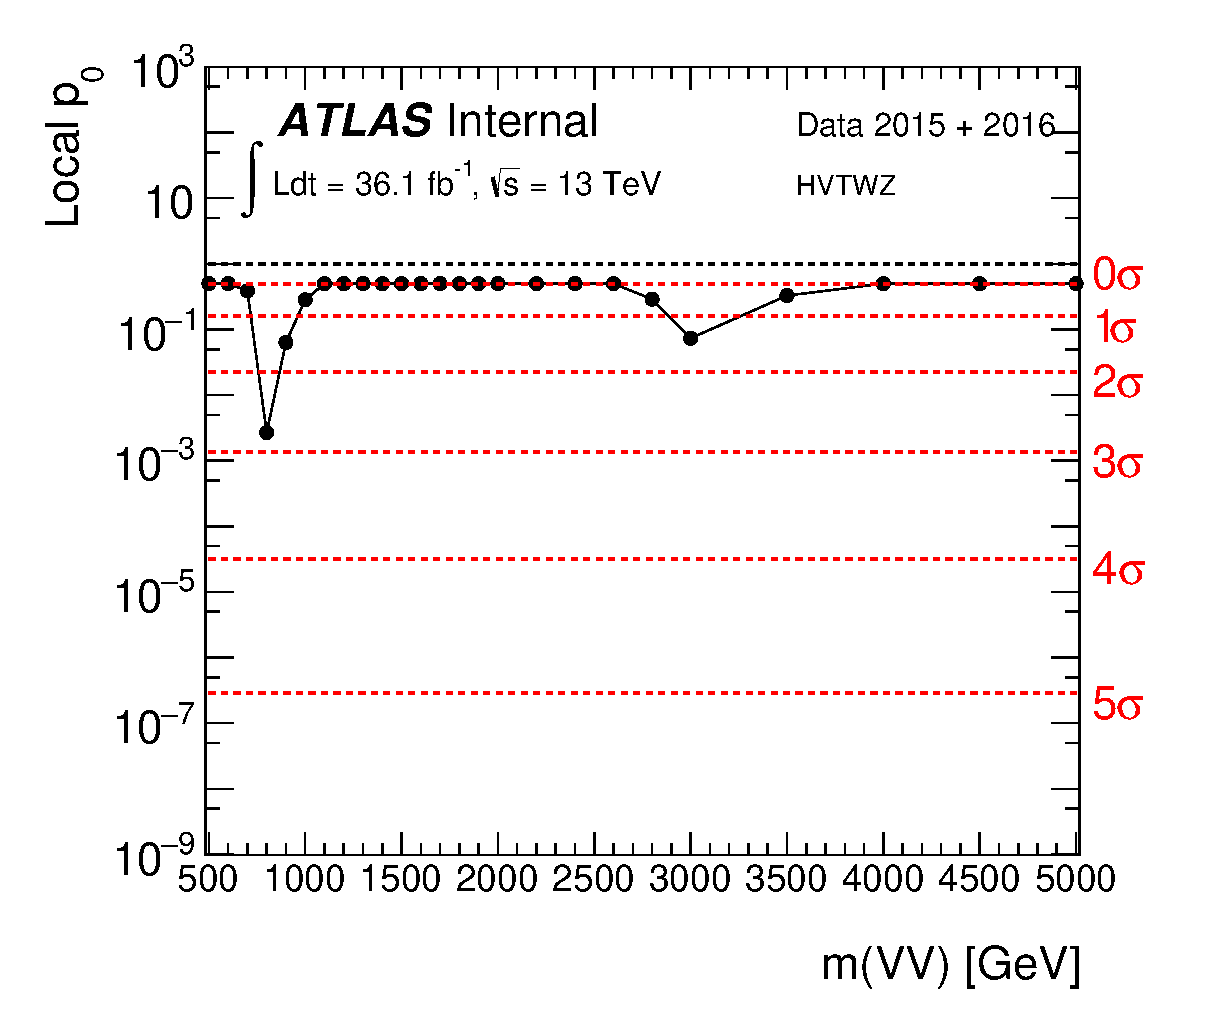
\includegraphics[width=0.75\textwidth]{Chapter4/VVM_p0_HVTWZ_ggF.eps}
	\caption{The observed p-value and significance for the W' boson from the ggF production with the combined data of both resolved and merged channels }
	\label{Fig:pvalue_hvt}
\end{figure}
\noindent
\\
\\{\bf Methodology for an Exclusion (Confidence Interval at $95\%$ Confidence Level)}
\\
\\Without a significant result ($Z<3\sigma$), an exclusion limit is then set to conclude that a specific range of theoretical hypotheses (i.e. new particles of varied mass range) has no signal which is within the analysis sensitivity (i.e. the particle production cross-section is significant to be measured). 
\\
\\In the case of an exclusion, an alternative test statistic is formulated as:
\begin{equation}
\tilde{q}_{\mu} = 
\begin{cases}
-2 \ln \lambda(\mu) & 0 \le \hat{\mu} \le \mu \\
0 & \hat{\mu} > \mu \\
-2 \ln \lambda(0) & \hat{\mu} < 0 \\
\end{cases}
\label{Eq:Sig_testQ}
\end{equation}
For the three cases in the expression, the bottom one is to keep $\mu$ positive to have physical meaning, when $\hat{\mu}$ is smaller than 0. For the other two cases, it is to have the $\mu$ hypothesis at one side for $\mu>\hat{\mu}$ which is to set the exclusion upper limit on the cross-section, and the lower limit is ignored. 
\\
\\Then, the asymptotic approach is applied again. Under this case, $\tilde{q}_{\mu}^{*}$ is chosen with the Asimov data to make:
\begin{equation}
p_{\mu}=\int_{\tilde{q}_{\mu}^{*}}^{\infty}f(\tilde{q}_{\mu}|\mu=0)\operatorname{d}\tilde{q}_{\mu}=0.05
\end{equation}
\noindent
This is meaning that if the signal exists with a specific signal strength, $\mu^*$, the null hypothesis would be rejected at $95\%$ confidence level (CL). Followed by that, $\mu^*$ is taken as the median value for the new p.d.f., $f(\tilde{q}_{\mu}|\mu=\mu^*)$, and also the expected upper limit of sensitivity to measure the signal. Then, the observed sensitivity is estimated to be the $\mu$ in this new p.d.f. corresponding to the observed event yield. This would lead to the claim that there is no signal with the given upper limit on cross-section at $95\%$ confidence, and there is still $5\%$ chance of the occurrence of the ``type II error'' which means to miss the signal within the expected sensitivity. 
\\
\\The final result is then interpreted by converting the evaluated $\mu$ into the production cross-section and the decay branch ratio:
\begin{equation}
\sigma\times BR=\frac{\mu\times N^{evt}}{\mathcal{L}}
\end{equation}  
with $\mathcal{L}$ as the luminosity
\\
\\The results with the combination of all the signal regions are presented in Fig.~ \ref{Fig:limit_ggF} for the ggF category with theoretical cross-section overlaid together, and Fig.~\ref{Fig:limit_VBF} for the VBF category. For the W' boson, Z' boson, and the RS graviton, the theoretical cross-section is overlaid together with the expect and observed limits from the experiment which presents that the measurement has the sensitivity on the mass up to $3~TeV$, and $1.7~TeV$ for the HVT bosons and gravitons respectively. And, Fig.~\ref{Fig:limit_comp_lvqq} shows the comparison of power to set a limit on the HVT Z' boson between resolved, merged, and combined channels. For the range of low mass, resolved channel has dominated the sensitivity, while for $m_{WV}>800~GeV$, merged channel has made better performance in terms of the sensitivity.

\begin{figure}[ht]
	\centering
	\subfloat[]{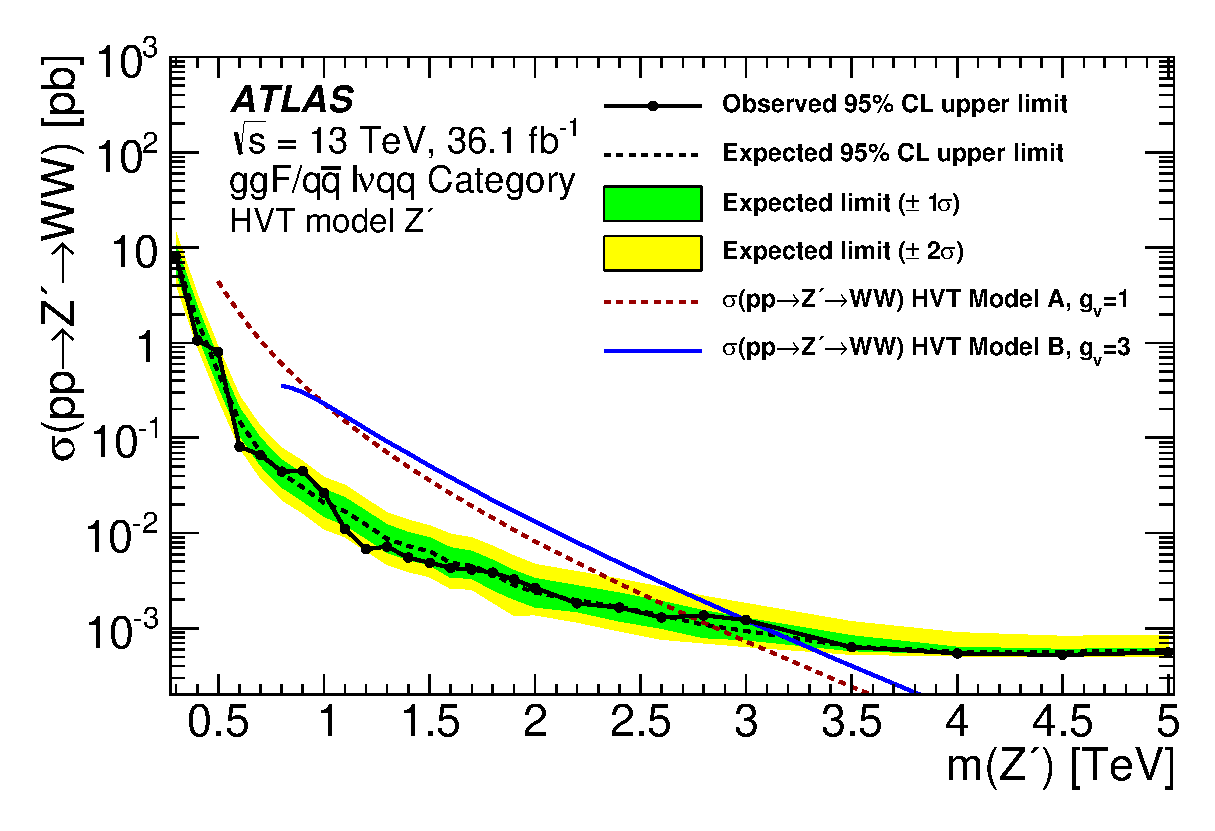
\includegraphics[width=0.5\textwidth]{Chapter4/GGFWWHVT.eps}}
	\subfloat[]{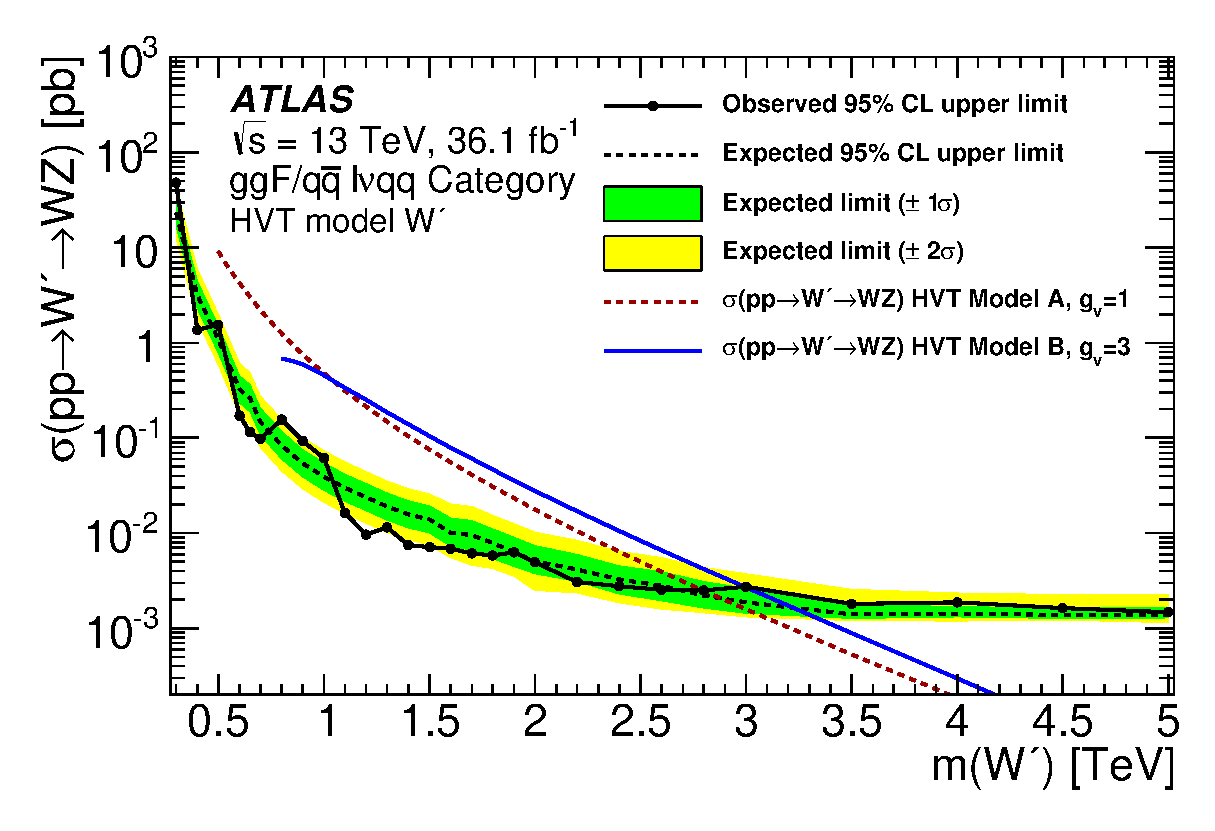
\includegraphics[width=0.5\textwidth]{Chapter4/GGFWZHVT.eps}}\\
	\subfloat[]{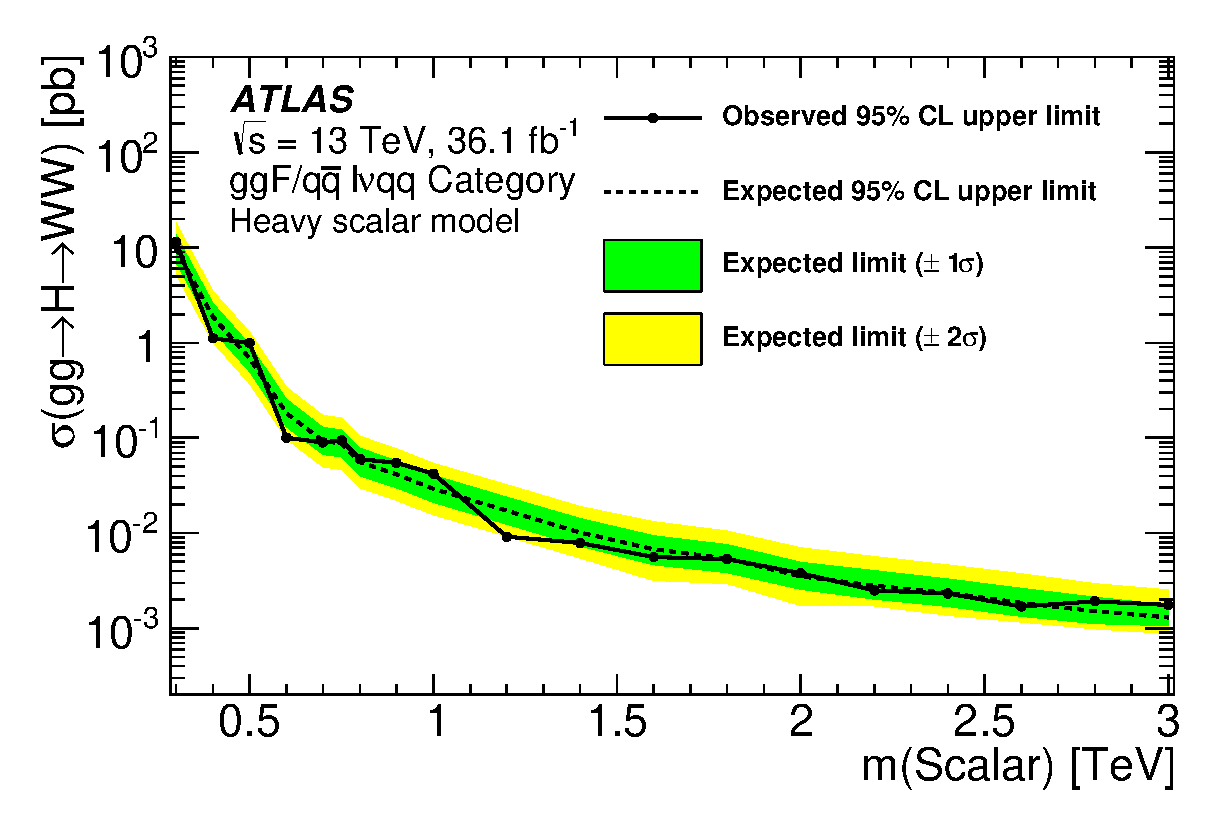
\includegraphics[width=0.5\textwidth]{Chapter4/GGFWWNWA.eps}}
	\subfloat[]{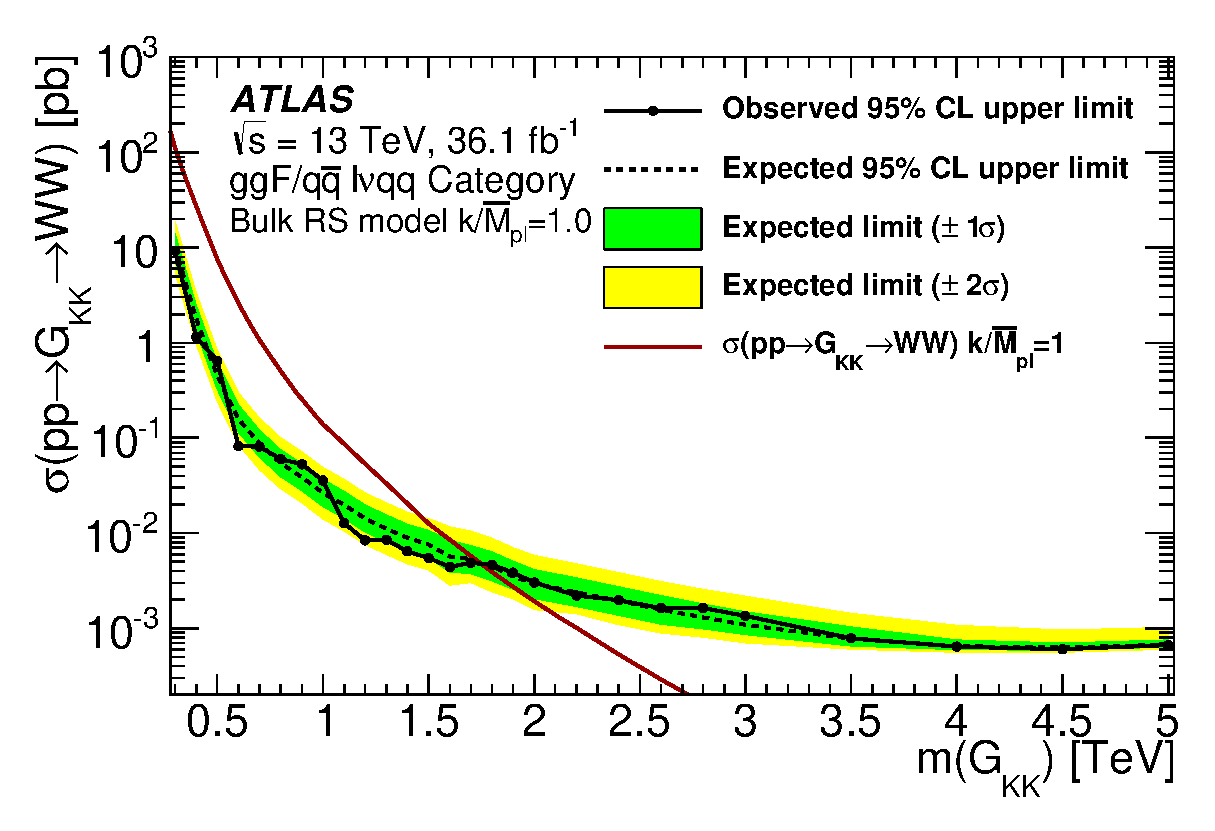
\includegraphics[width=0.5\textwidth]{Chapter4/GGFWWRSG.eps}}
	\caption{The limits for the BSM particles via ggF/DY production. (a) and (b) are for the HVT Z' and W' bosons, while (c) is for the NWA scalar boson, and (d) is for the RS graviton.}
	\label{Fig:limit_ggF}
\end{figure}
\begin{figure}[ht]
	\centering
	\subfloat[]{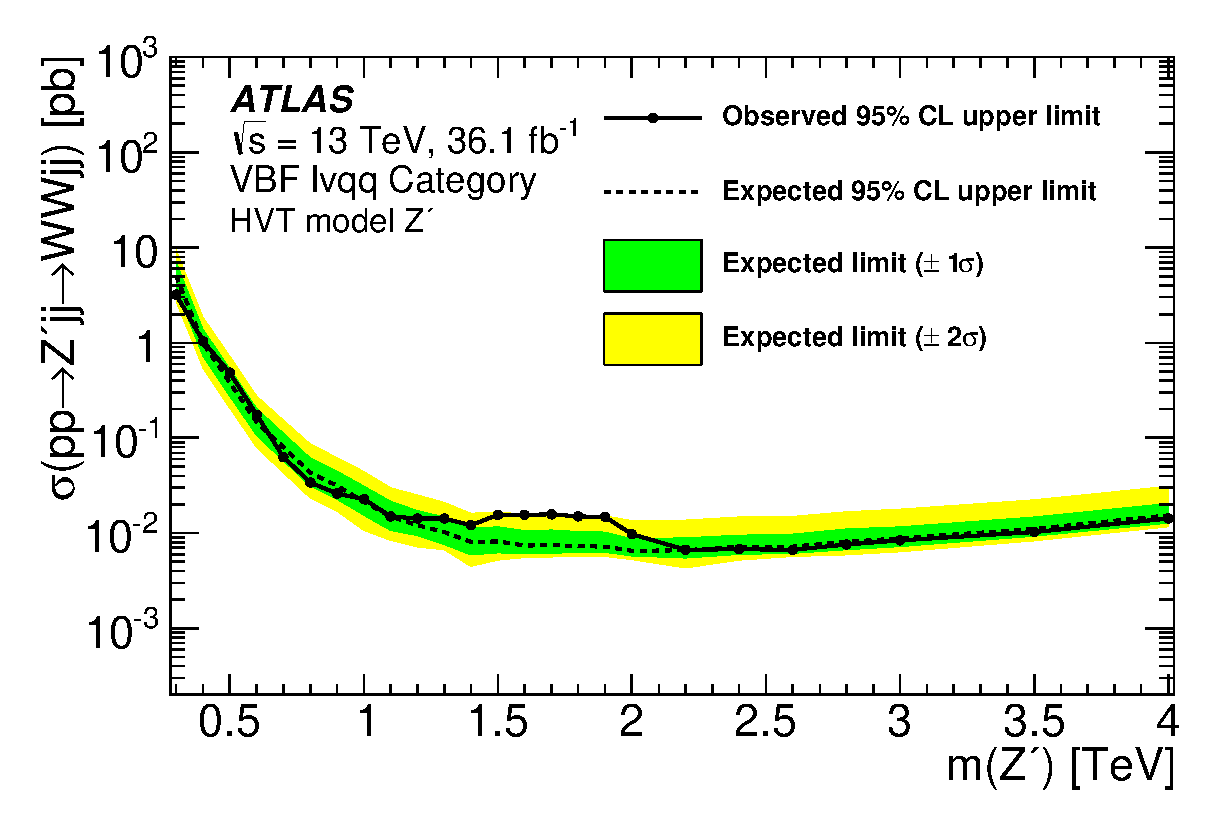
\includegraphics[width=0.5\textwidth]{Chapter4/VBFWWHVT.eps}}
	\subfloat[]{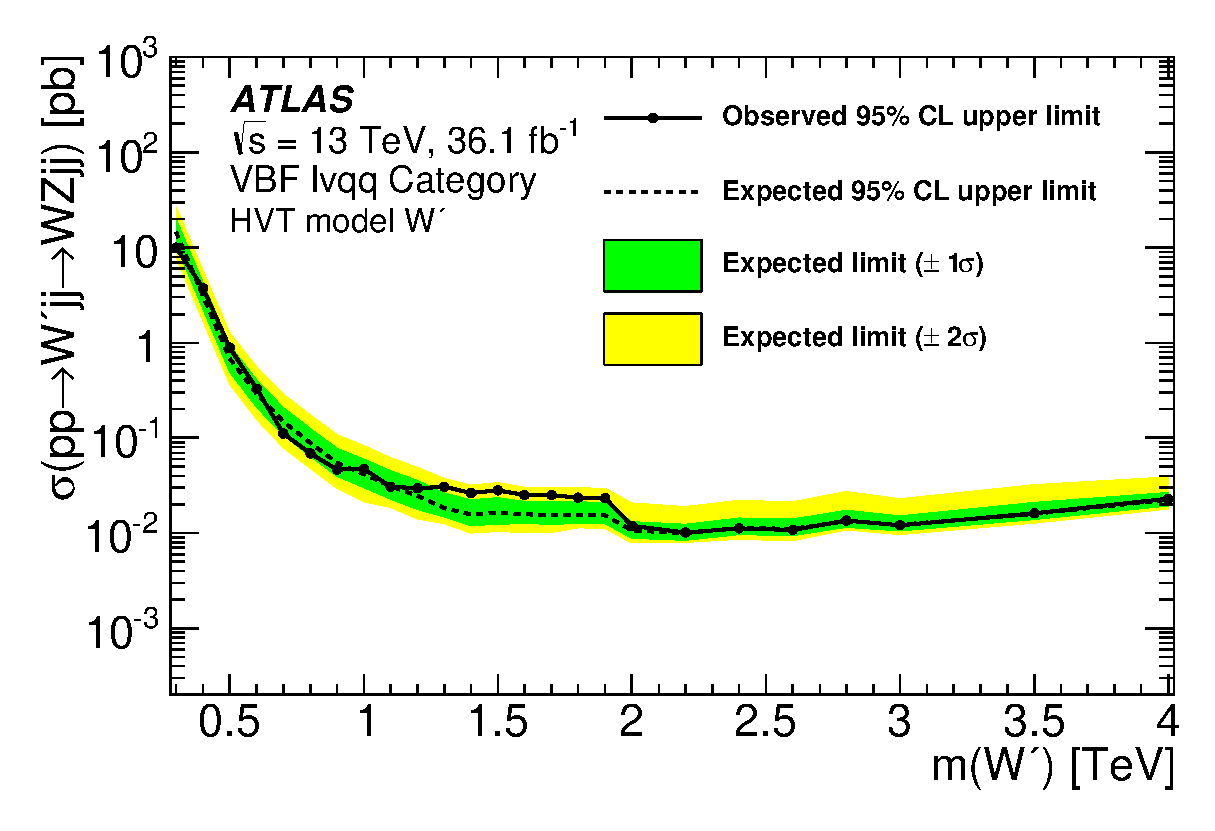
\includegraphics[width=0.5\textwidth]{Chapter4/VBFWZHVT.eps}}\\
	\subfloat[]{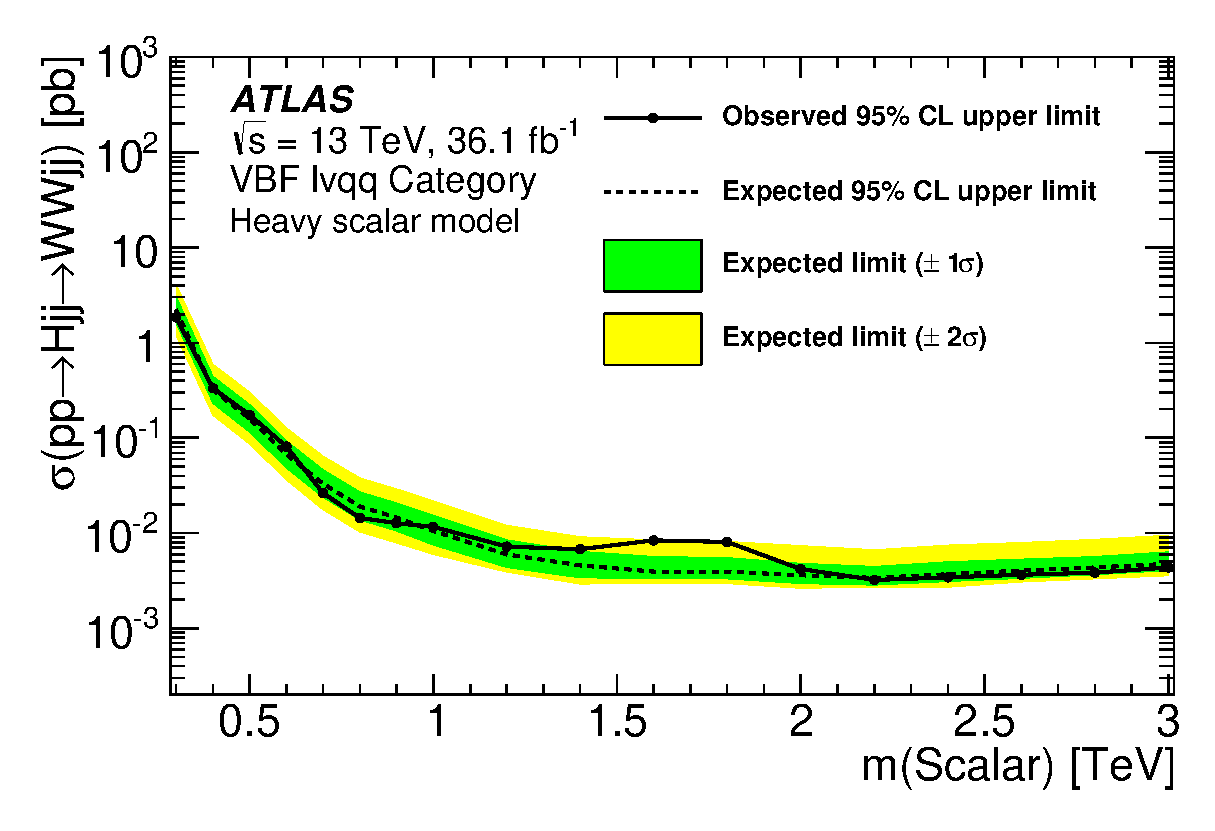
\includegraphics[width=0.5\textwidth]{Chapter4/VBFWWNWA.eps}}
	\caption{The limits for the BSM particles via VBF production. (a) and (b) are for the HVT Z' and W' bosons, while (c) is for the NWA scalar boson. For the RS graviton, the VBF production is not considered}
	\label{Fig:limit_VBF}
\end{figure}
\begin{figure}[ht]
	\centering
	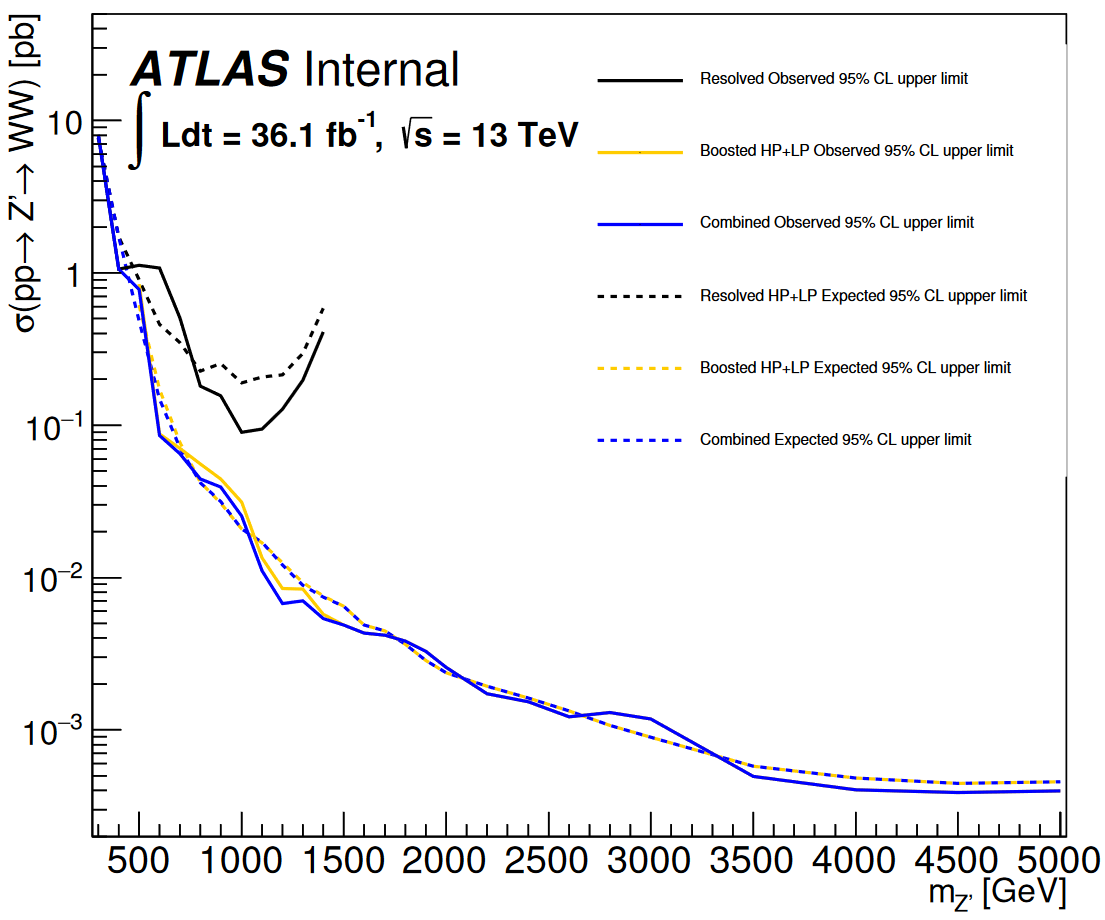
\includegraphics[width=0.8\textwidth]{Chapter4/limit_ResMerComb.png}
    \caption{The limit comparison between the merged, resolved, and combined channels.}
    \label{Fig:limit_comp_lvqq}
\end{figure}
\section{Combination of VV/VH/$\ell\ell$/$\ell\nu$}
As mentioned before, the combination of multiple signal regions would help to increase the statistics and improve the measured sensitivity.  In addition to the final state this analysis is interested in($pp\to WV \to \ell\nu qq$), there are also other analyses which are aiming for the same exotic particles. Therefore, a combination across all the possible final states of those searches was conducted to have a further improvement in the final result. The proposed scheme is to combine the diboson analyses for which the final states of VV (V=W or Z boson) decay are considered to search for the scalar NWA boson, the HVT, and the RS graviton. And, to have a further understanding of the HVT coupling to the SM particles, the dilepton ($\ell\ell$ and $\ell\nu$) and VH ($H\to bb$) channels are also taken into the combination.
\\
\\The discriminant used in the combination is the fully reconstructed mass, $m_{WV}$, and the transverse mass, $m_{T}$ is taken when the mass could not be fully reconstructed. (like $VV\to\nu\nu\ell\ell$ or $X\to\ell\nu$).
\\
\\As discussed in the last chapter, the signal configuration was set to have a narrow resonance mass window, so the effect of interference on the cross-section is smaller than $15\%$ in the VV and VH channels. Therefore, interference is taken to be negligible. For the dilepton channel, a cut on the resonance (transverse) mass is applied to mitigate the effect. \cite{EXOT-2018-01} 
\subsection{Combination Strategy}
The combination scheme could be seen in Fig. \ref{Fig:Comb_scheme}, and the considered analyses with a brief event selection summary is presented in Tab. \ref{tab:signatures}.
\begin{figure}[ht]
	\centering
	\subfloat[]{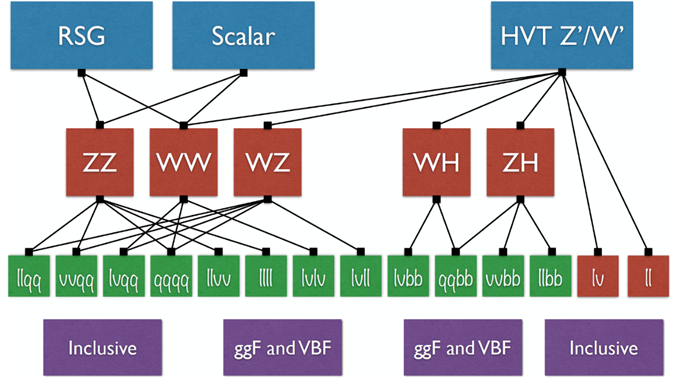
\includegraphics[width=0.9\textwidth]{Chapter4/Comb_scheme.png}}
	\caption{The scheme for combination of VV, VH, and dilepton analyses with their final states. It could be seen that decays channels for WW, WZ, ZZ, WH, and ZH are combined respectively first. Then, the further combinations are performed to give the final interpretation.}
	\label{Fig:Comb_scheme}
\end{figure}


\begin{table}[t]
	\caption{The list of individual analyses which are taken into the combination}
	\begin{center}
		\begin{tabular}{l l c c c c c c}
			\hline
			Channel            & Diboson state & \multicolumn{4}{c}{~~~~~~Selection}       & VBF cat. & Reference \\
			&               & Leptons       & $E^{miss}_T$  & Jets   & $b$-tags &          &           \\
			\hline
			$qq qq$            & $WW/WZ/ZZ$    & 0             & veto  & 2J     & $-$      & $-$      & \cite{EXOT-2016-19} \\
			$\nu\nu qq$        & $WZ/ZZ$       & 0             & yes   & 1J     & $-$      & yes      & \cite{EXOT-2016-29} \\
			$\ell\nu qq$       & $WW/WZ$       & $1e, 1\mu$    & yes   & 2j, 1J & $-$      & yes      & \cite{EXOT-2016-28} \\
			$\ell\ell qq$      & $WZ/ZZ$       & $2e, 2\mu$    & $-$   & 2j, 1J & $-$      & yes      & \cite{EXOT-2016-29} \\
			$\ell\ell\nu\nu$   & $ZZ$          & $2e, 2\mu$    & yes   & $-$    & 0        & yes      & \cite{HIGG-2016-19} \\
			$\ell\nu\ell\nu$   & $WW$          & $1e$+$1\mu$   & yes   & $-$    & 0        & yes      & \cite{HIGG-2016-31} \\
			$\ell\nu\ell\ell$  & $WZ$          & $3e$, $2e$+$1\mu$, $1e$+$2\mu$, $3\mu$ & yes & $-$ & 0 & yes & \cite{EXOT-2016-11} \\
			$\ell\ell\ell\ell$ & $ZZ$          & $4e$, $2e$+$2\mu$, $4\mu$ & $-$ & $-$ & $-$ & yes    & \cite{HIGG-2016-19} \\
			\hline
			$qq bb$            & $WH/ZH$       & 0             & veto  & 2J     & 1, 2     & $-$      & \cite{EXOT-2016-12} \\
			$\nu\nu bb$        & $ZH$          & 0             & yes   & 2j, 1J & 1, 2     & $-$      & \cite{EXOT-2016-10} \\
			$\ell\nu bb$       & $WH$          & $1e, 1\mu$    & yes   & 2j, 1J & 1, 2     & $-$      & \cite{EXOT-2016-10} \\
			$\ell\ell bb$      & $ZH$          & $2e, 2\mu$    & veto  & 2j, 1J & 1, 2     & $-$      & \cite{EXOT-2016-10} \\
			\hline
			$\ell\nu$          & $-$           & $1e, 1\mu$    & yes   & $-$    & $-$      & $-$      & \cite{EXOT-2016-06} \\
			$\ell\ell$         & $-$           & $2e, 2\mu$    & $-$   & $-$    & $-$      & $-$      & \cite{EXOT-2016-05} \\
			\hline
		\end{tabular}
		\label{tab:signatures}
	\end{center}
\end{table}


\noindent
\\With the number of involved analyses, the likelihood construction of all the final state would be too complicated, so the procedure was conducted step by step. It started from the combination of channels with same medium states of WW, WZ, or ZZ bosons. For example, there are three analyses involved for $X\to WW$ with final states of $\ell\nu qq$, $\ell\nu\ell\nu$ and qqqq, so they are combined first.Then, the combined results of WW, WZ, and ZZ are further combined to give the VV combination result. At this stage, the statistic interpretations for RS gravitons and NWA scalar bosons are completed. Following by that, the VV channels are combined together with VH and dilepton channels to set the limit on mass of W' and Z' bosons as well as the coupling strength between the HVT and SM particles.  
\\
\\{\bf Orthogonality }
\\
\\Within VV and VH channels, the category orthogonality was kept by the cuts on lepton number, $E^{miss}_T$, and b-jet numbers. However, due to overlapped mass windows between W/Z and Higgs bosons, some events went into both VV and VH signal regions. Tab. \ref{Tab:VVVH_masswindow} shows the mass windows used in the hadronically decayed bosons. In this case, the events are given higher priority to go into the VV category and get removed from the VH channels, if the selected dijet system has the mass in the overlapped region. With the comparison to the original event selection, the expected sensitivity does not have significant change ($<10\%$) which could be seen in Fig. \ref{Fig:limits_Hbb}. 
\begin{table}
	\caption{The mass windows for the selection on hadronically decayed bosons in VV and VH events}
	\label{Tab:VVVH_masswindow}
	\begin{tabular}{c|c|c|c|c}
		\hline
		channel                                    & Jet Topo  & W       &    Z     &  H \\
		\hline
		\hline
		\multirow{ 2}{*}{$qqqq$}                   & resolved  & - & - &  - \\
		\cline{2-5}
                                                   & merged    & [65,95] & [76,106] &  - \\
		\hline
		\multirow{ 2}{*}{$\ell\ell qq$}            & resolved  & [62,97] & [70,105] &  - \\
		\cline{2-5}
                                                   & merged    & [65,95] & [76,106] &  - \\
		\hline 
		\multirow{ 2}{*}{$\ell\nu qq$}             & resolved  & [66,94] & [82,106] &  - \\
		\cline{2-5}
                                                   & merged    & [64,104](LP) & [69,114](LP) &  - \\
		\hline
		\multirow{ 2}{*}{$\nu\nu qq$}              & resolved  & - & - &  - \\
		\cline{2-5}
                                                   & merged    & [65,95] & [76,106] &  - \\
		\hline 
		\multirow{ 2}{*}{$qqbb$}                   & resolved  & - & - &  - \\
		\cline{2-5}
                                                   & merged    & - & [70,110] (HP) &  [75,145] \\
		\hline 
		\multirow{ 2}{*}{$\ell\nu bb$/$\nu\nu bb$} & resolved  & \multicolumn{3}{c}{[110,140]} \\
		\cline{2-5}
                                                   & merged    & \multicolumn{3}{c}{[75,145]} \\
	    \hline
		\multirow{ 2}{*}{$\ell\ell bb$}            & resolved  & \multicolumn{3}{c}{[100,145]} \\
        \cline{2-5}
                                                   & merged    & \multicolumn{3}{c}{[75,145]} \\
        \hline
	\end{tabular}
\end{table} 
\begin{figure}[ht]
	\centering
	\subfloat[]{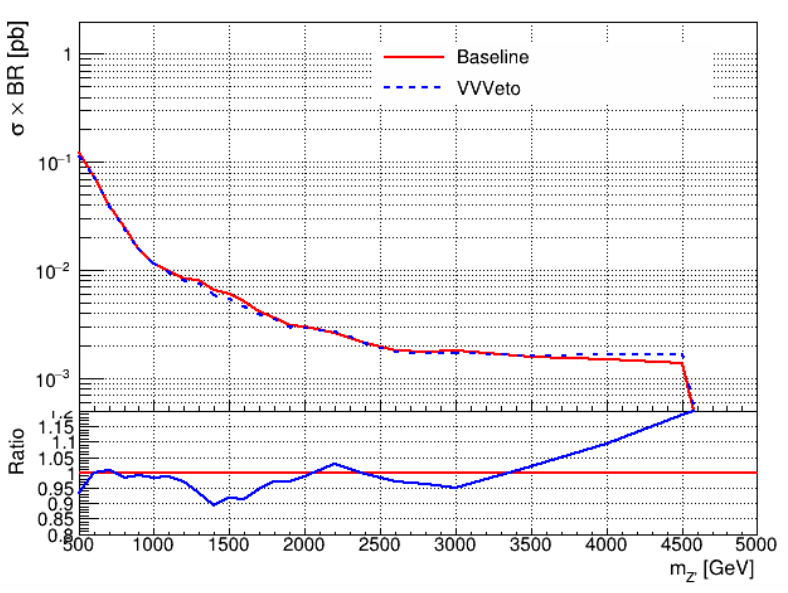
\includegraphics[width=0.34\textwidth]{Chapter4/vvbb_limit.png}}
	\subfloat[]{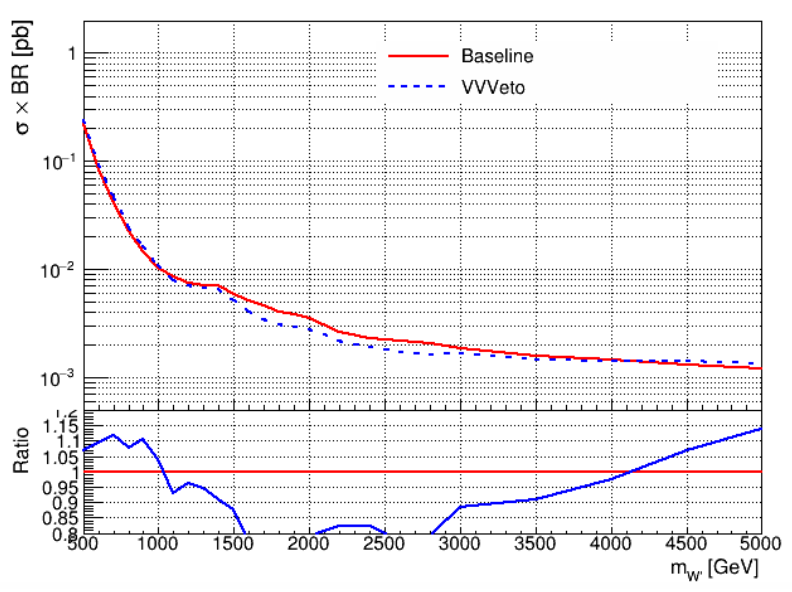
\includegraphics[width=0.34\textwidth]{Chapter4/lvbb_limit.png}}	\subfloat[]{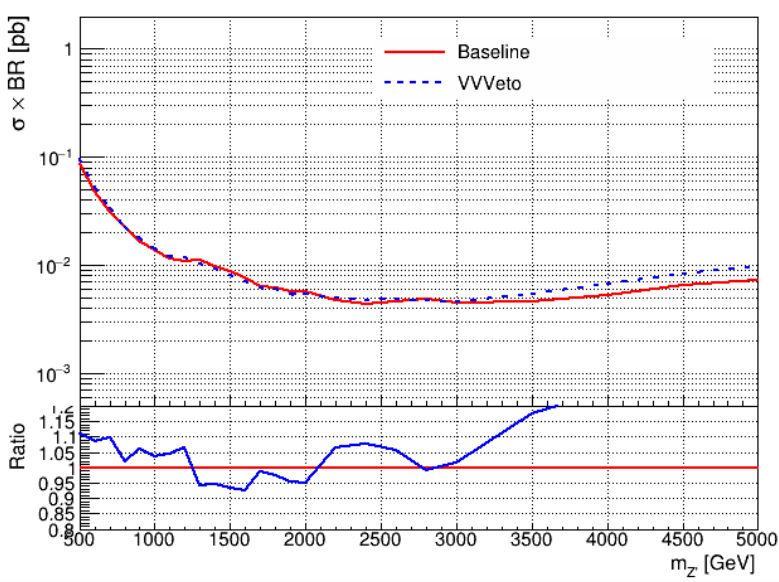
\includegraphics[width=0.34\textwidth]{Chapter4/llbb_limit.png}}
	\caption{The change in expected limits in the VH channels for (a)$VH\to\nu\nu bb$ (b)$VH\to\ell\nu bb$ and (c) $VH\to\ell\ell bb$ }
	\label{Fig:limits_Hbb}
\end{figure}
\noindent
\\
\\{\bf Nuisance Parameter Correlation}
\\
\\For each individual analysis, more than 100 nuisance parameters are considered. Some of them are commonly applied across the analyses, but there are also the ones which only made the contribution to the dedicated analyses. The following is the list of nuisance parameters which are decorrelated from the other analyses:
\begin{itemize}
	\item[] {\bf Jet Uncertainties}: The measurement of jets actually have 81 sources of uncertainties, but most of analyses just deploy the simplified schemes for which the 81 sources are combined into 21 or 3 uncertainties. For the analyses using different simplified uncertainty schemes, their jet uncertainties are uncorrelated ($VV\to\ell\nu\ell\ell\&\ell\ell\nu\nu$)
	\item[] {\bf Electron ID Uncertainty}: The  $VV\to\ell\nu\ell\nu$ analysis has deployed different identification working points in the electron selection, so the related uncertainties are uncorrelated. 
	\item[] {\bf Signal and Background Modelling Uncertainties}: The scale factors for the SM background in the likelihood reconstructions are decorrelated as they have different kinematic properties for varied final states. Furthermore, the uncertainties arising from the data-driven estimation are also decorrelated. As the ISR and FSR effect was not considered in the fully leptonically decayed channels, they are uncorrelated as well.  
\end{itemize}
\subsection{Result}
The combination is aiming for two kinds of results: the limit on the mass of exotic partices (NWA scalar boson, HVT W' and Z' bosons, and RS gravtion), and the limit on the coupling strength between the HVT and SM particles. The first result will follow the asymptotic methodology which was discuss in Sec.\ref{Sec:lvqq_result} with a cross-check from the toy model\footnote{as running the toy model is computationally expensive, it it only performed on the mass points of 1, 2, 3, 4, and 5 TeV}, and , for the second result, a similar likelihood would be constructed by the parameter of interest would be the coupling constant, $\vec{g}$, instead of the signal strength, $\mu$. The detail will be coming later. 
\\
\\{\bf Mass Limits}
\\
\\The cross-section limits are set with the ggF/DY and VBF productions respectively. For the VBF category, not all analyses have this channel, but they are still combined to provide the upper limit, and the results are shown in Fig.~\ref{Fig:limit_VBF_comb}. Here, a new benchmark for the HVT model is applied with $g_{H}=1$ and $g_{f}=0$, and this means the production of W' and Z' bosons could only be via VBF. With this new configuratio (named as model c), the sensitivity is set as the inclusive (W' + Z' bosons) cross-section upper limit ratio between the expectation (observation) and theory. With respect to the single channel analysis presented before, the mass limit has seen a significant improvement from $1.2~TeV$($3~TeV$) to $2.2~TeV$($4.5~TeV$) for the RS graviton (HVT boson) interpretation.   
\begin{figure}[ht]
	\centering
	\subfloat[]{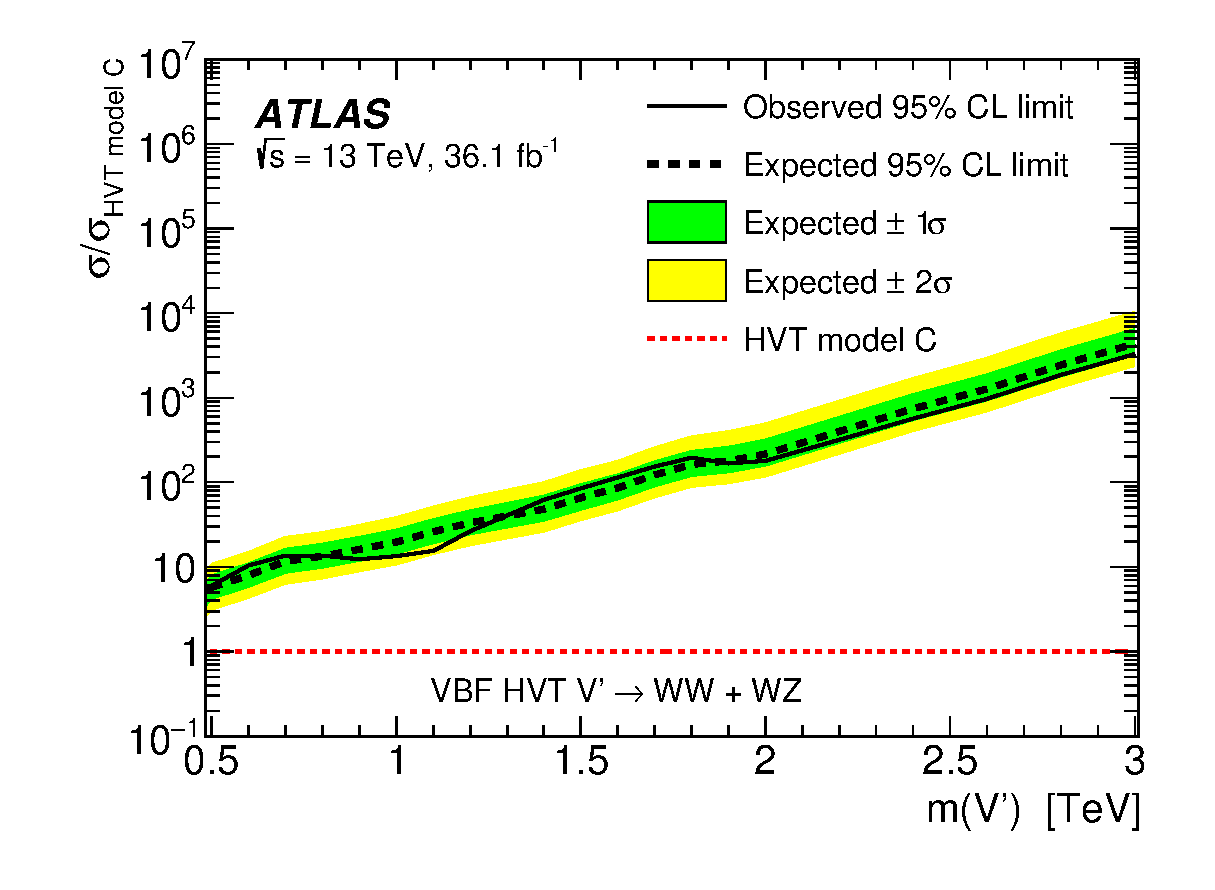
\includegraphics[width=0.5\textwidth]{Chapter4/VBFWWWZHVT_COMB.eps}}
	\subfloat[]{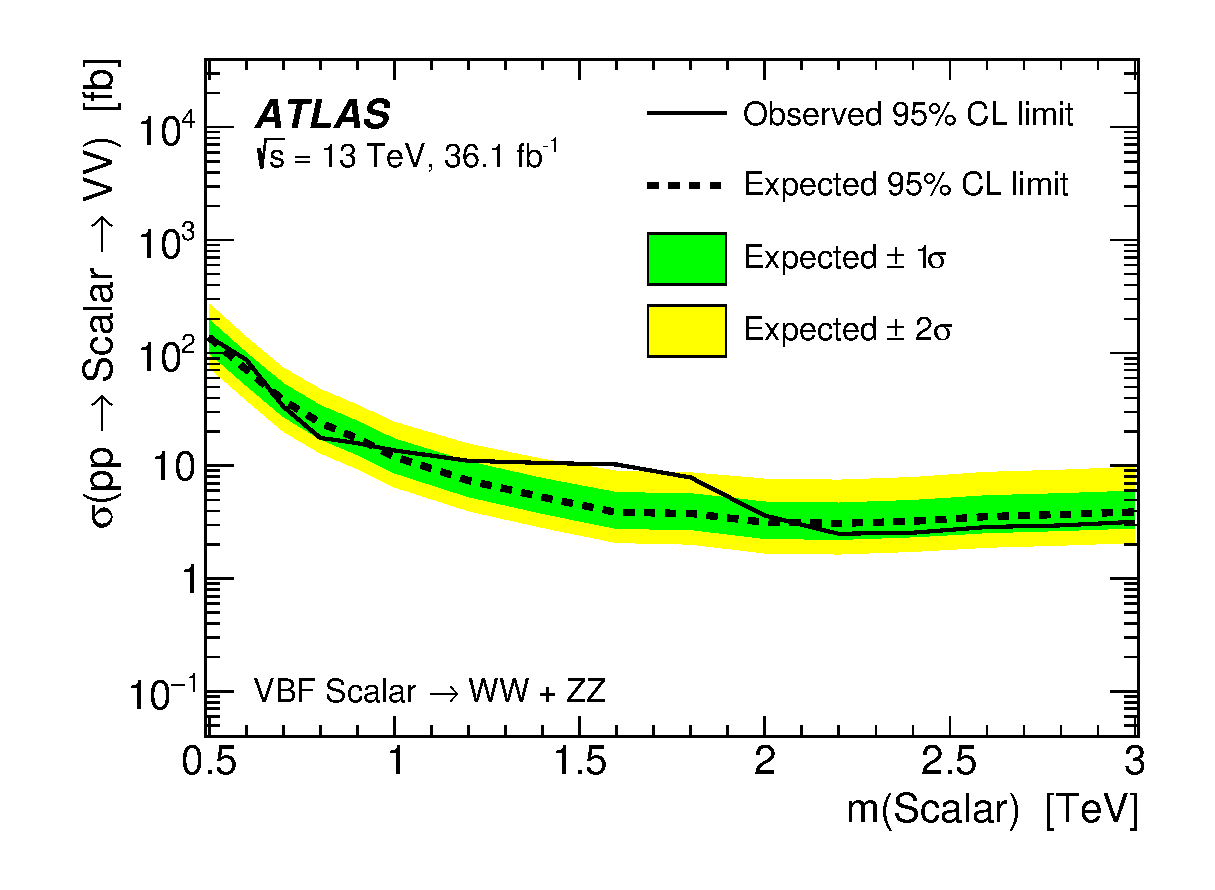
\includegraphics[width=0.5\textwidth]{Chapter4/VBFWWZZNWA_COMB.eps}}
	\caption{The cross-section upper limit for (a) the HVT model boson (as a ratio to the theoretical one) (b) and the NWA scalar boson }
	\label{Fig:limit_VBF_comb}
\end{figure}
\noindent
\\
\\For the ggF result, the VV channel is combined with VH and dilepton channels for the HVT interpretation, while the limits on models of RS graviton and NWA scalar boson are only set with the VV channel. The HVT interpretation is shown in Fig.~\ref{Fig:limit_GGFHVT_comb} as the ratio of the observed cross-section to the theoretically predicted cross-section. And, the limits on RS graviton and NWA scalar bosons are in Fig.~\ref{Fig:limit_GGF_comb}, while Fig.~\ref{Fig:limit_GGFHVTV_compare} is presenting the comparison of the sensitivities from the VV+VH and dilepton channels. 
\begin{figure}[ht]
	\centering
	\subfloat[]{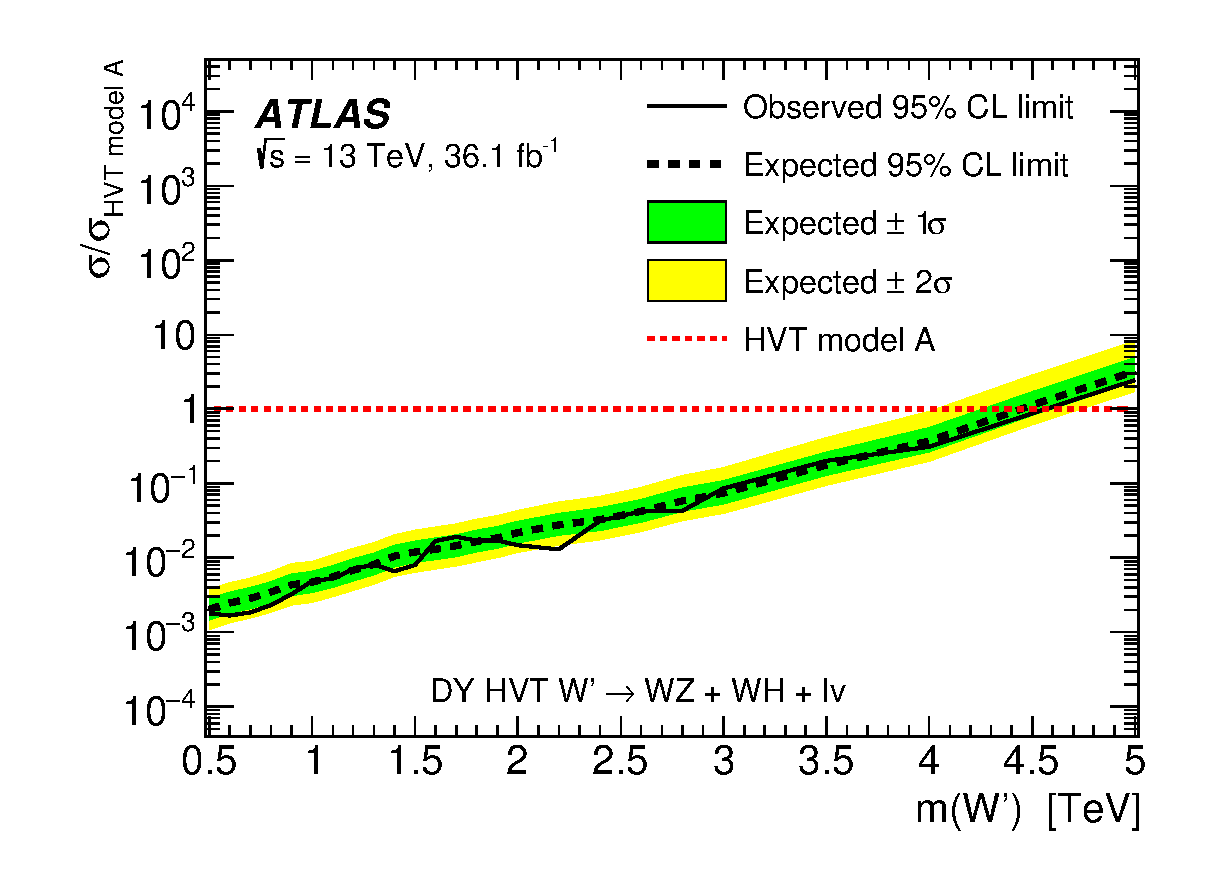
\includegraphics[width=0.5\textwidth]{Chapter4/GGFALLHVTW_COMB.eps}}
	\subfloat[]{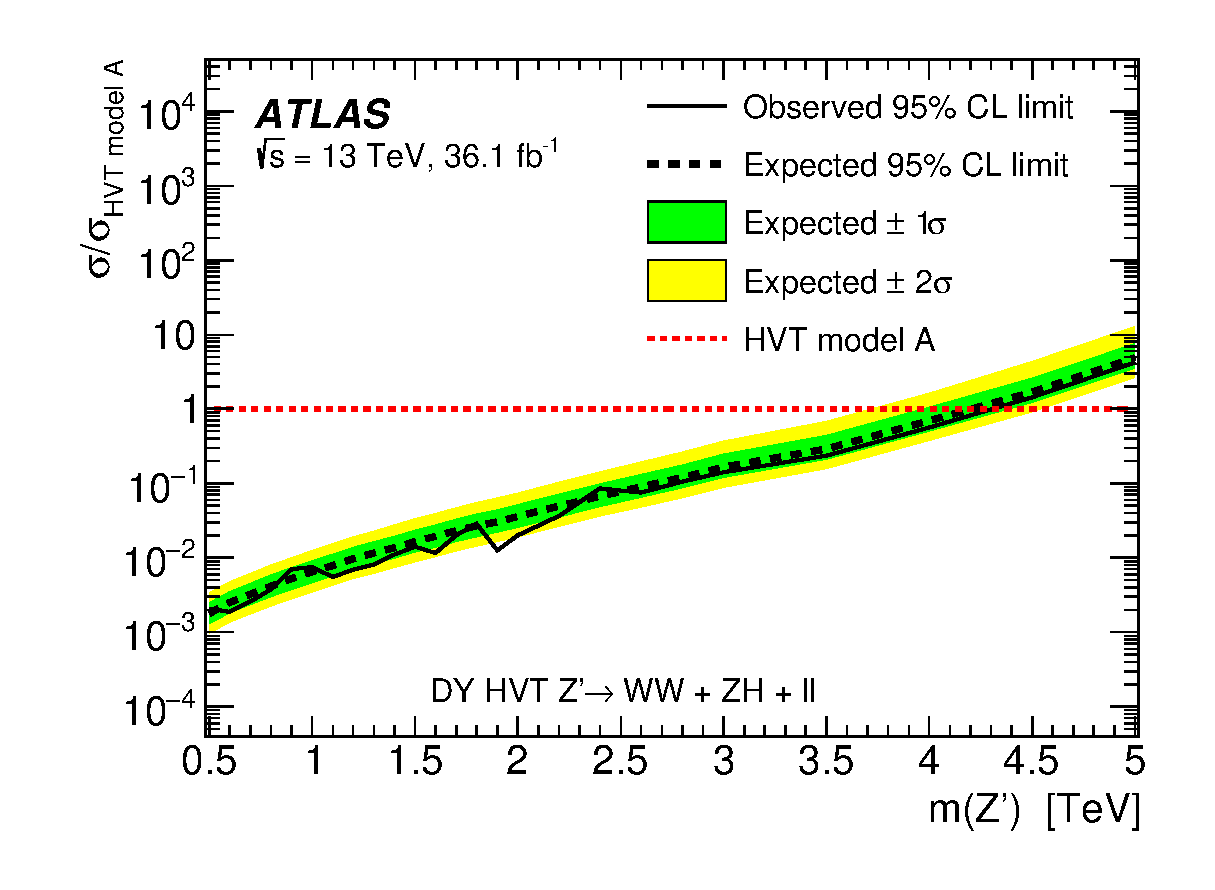
\includegraphics[width=0.5\textwidth]{Chapter4/GGFALLHVTZ_COMB.eps}}
	\caption{The cross-section upper limit ratio to the HVT model theoretical prediction for (a) the W' boson (b) the Z' boson }
	\label{Fig:limit_GGFHVT_comb}
\end{figure}
\begin{figure}[ht]
	\centering
	\subfloat[]{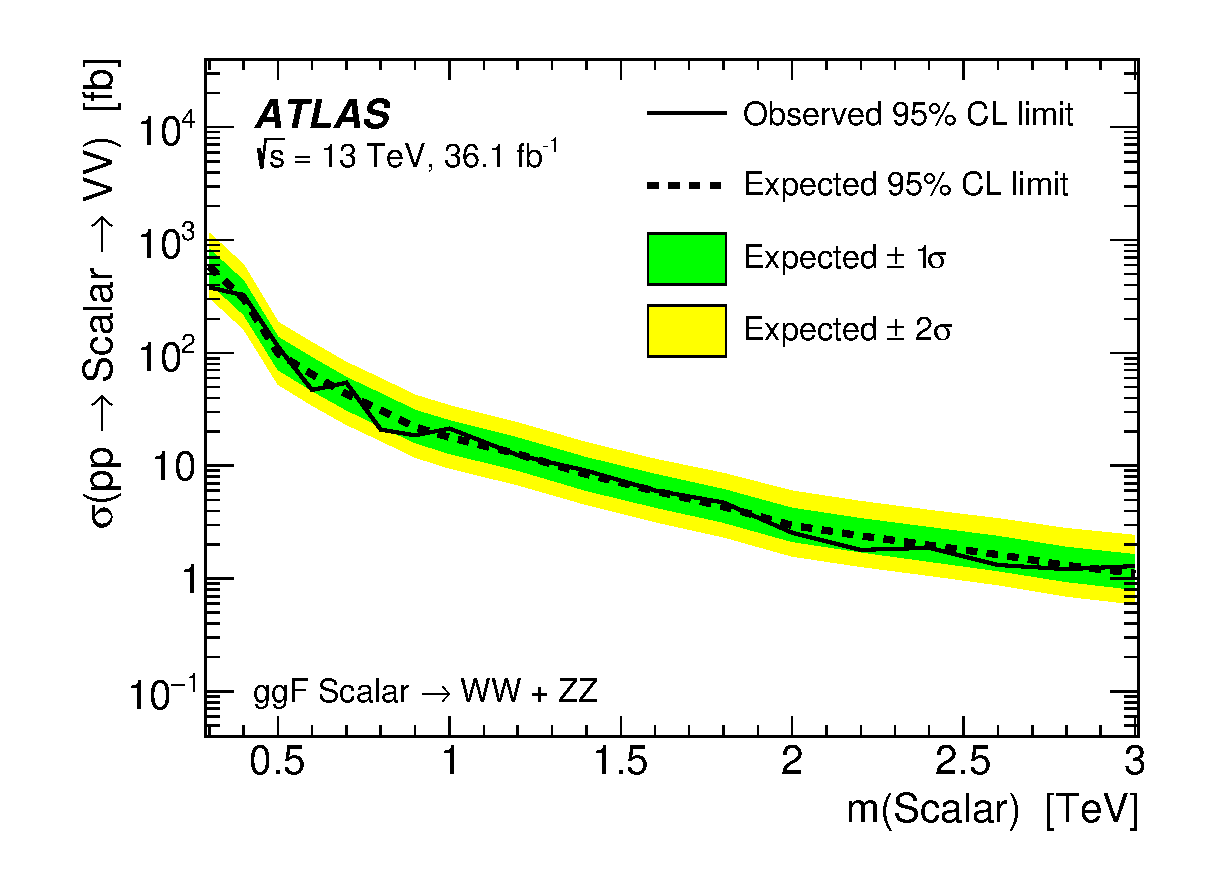
\includegraphics[width=0.5\textwidth]{Chapter4/GGFWWZZNWA_COMB.eps}}
	\subfloat[]{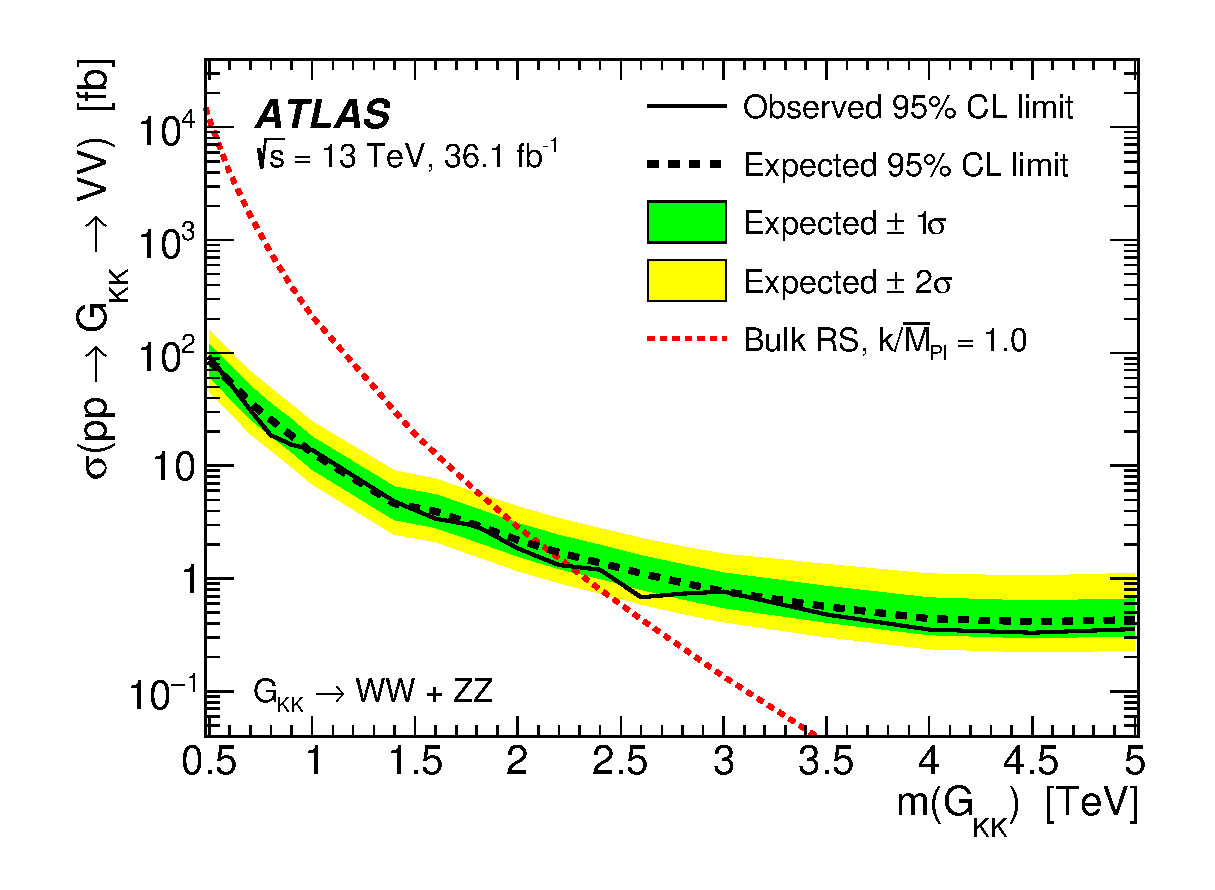
\includegraphics[width=0.5\textwidth]{Chapter4/GGFWWZZRSG_COMB.eps}}
	\caption{The cross-section upper limit on the (a) NWA scalar boson (b) RS graviton}
	\label{Fig:limit_GGF_comb}
\end{figure}
\begin{figure}[ht]
	\centering
    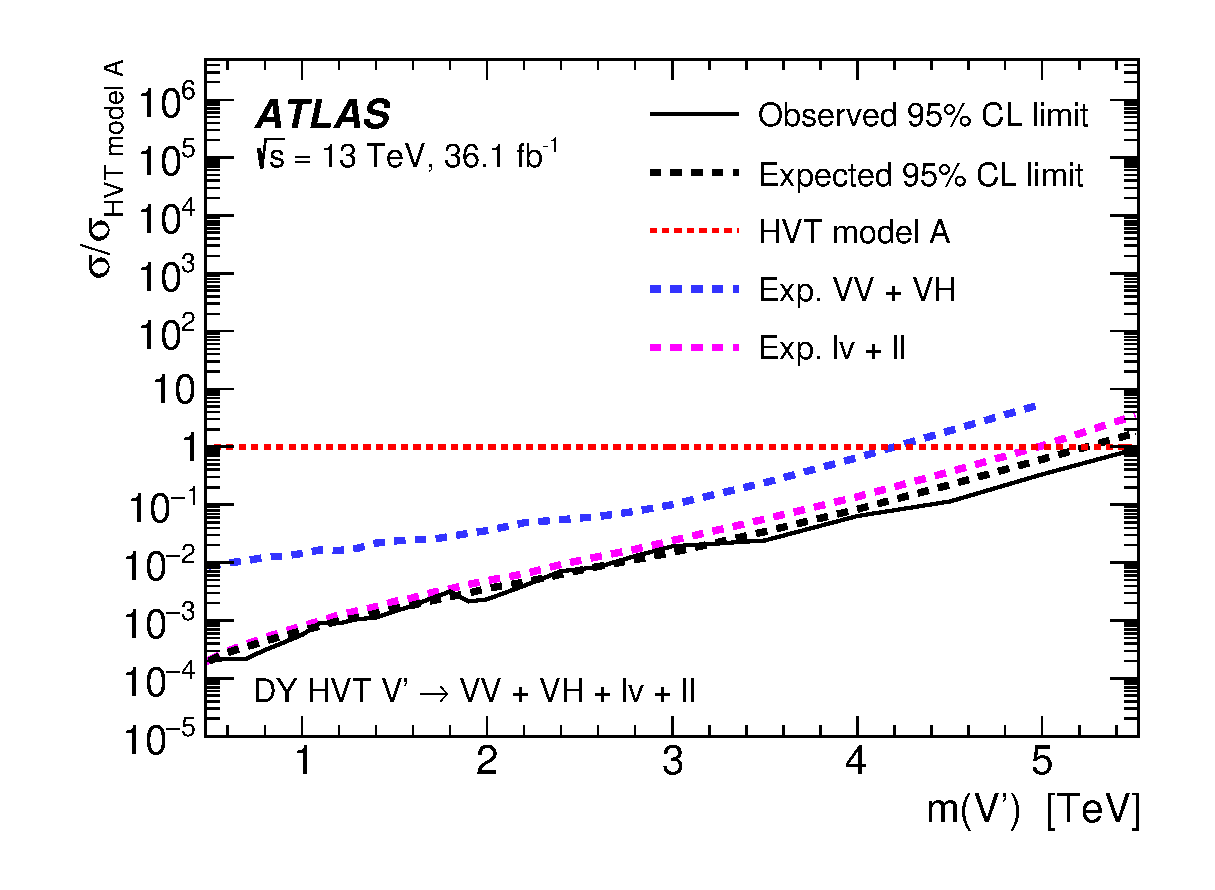
\includegraphics[width=0.5\textwidth]{Chapter4/GGFALLHVTV_compare.eps}
    \caption{The comparison on the limits on the HVT V' bosons set by different channels}
	\label{Fig:limit_GGFHVTV_compare}
\end{figure}
\noindent
\\
\\{\bf Coupling Limits}
\\
\\The limits of the HVT couplings are set on a two-dimensional plane with which two pairs of parameters are used:
\begin{itemize}
  \item[] {\bf $g_{H}$ and $g_{f}$}: they are corresponding to the couplings to the SM bosons (W, Z, and H) and fermions. For the simplicity, the fermionic coupling is set equal between quarks and leptons. 
  \item[] {\bf $g_{l}$ and $g_{q}$}: they are corresponding to the couplings to the leptons and quarks with the coupling to SM bosons set at 0.56 (model A).
\end{itemize}
\noindent
\\For the estimation of the couplings, the same method in Sec.\ref{Sec:lvqq_result} is applied with the profile likelihood and asymptotic formulae, but the likelihood is constructed with the coupling strengths, $\vec{\mathcal{G}}$ :
\begin{equation}
\lambda(\vec{\mathcal{G}}) = \frac{\mathcal{L}(\vec{\mathcal{G}},\hat{\hat{\theta}})}{\mathcal{L}(\hat{\vec{\mathcal{G}}},\hat{\theta})}
\end{equation}
Then, the event yields (signal strength) would be parametrized in terms of the couplings, and the following procedure is to set the exclusion limit at the $95\%$ confidence level .
\\
\\The final results are shown in Fig.~\ref{Fig:limit_coupling} on which the region outside dotted lines are excluded, and exclusions from the electroweak precision measurements \cite{delAguila:2010mx} are also overlaid as the coloured exclusion region which has combined the following experiments:
\begin{itemize}
	\item Z mass pole measurements from LEP\cite{delAguila:2010mx}
	\item LEP2 measurements provided in the last joint paper by the ALEPH, DELPHI, L3, and OPAL Collaborations\cite{Schael:2013ita}
	\item Measurements from low-energy experiments, CKM unitarity and $\alpha_{s}$\cite{Olive_2016}
	\item World average for the top-quark mass measurements from the ATLAS, CMS, CDF, and D0 Collaborations\cite{ATLAS:2014wva}
	\item World average for the Higgs boson mass measurements with Run 1 data from the ATLAS and CMS Collaborations (the cross-section measurement is not included)\cite{Aad:2015zhl}
\end{itemize}
\begin{figure}[ht]
	\centering
	\subfloat[]{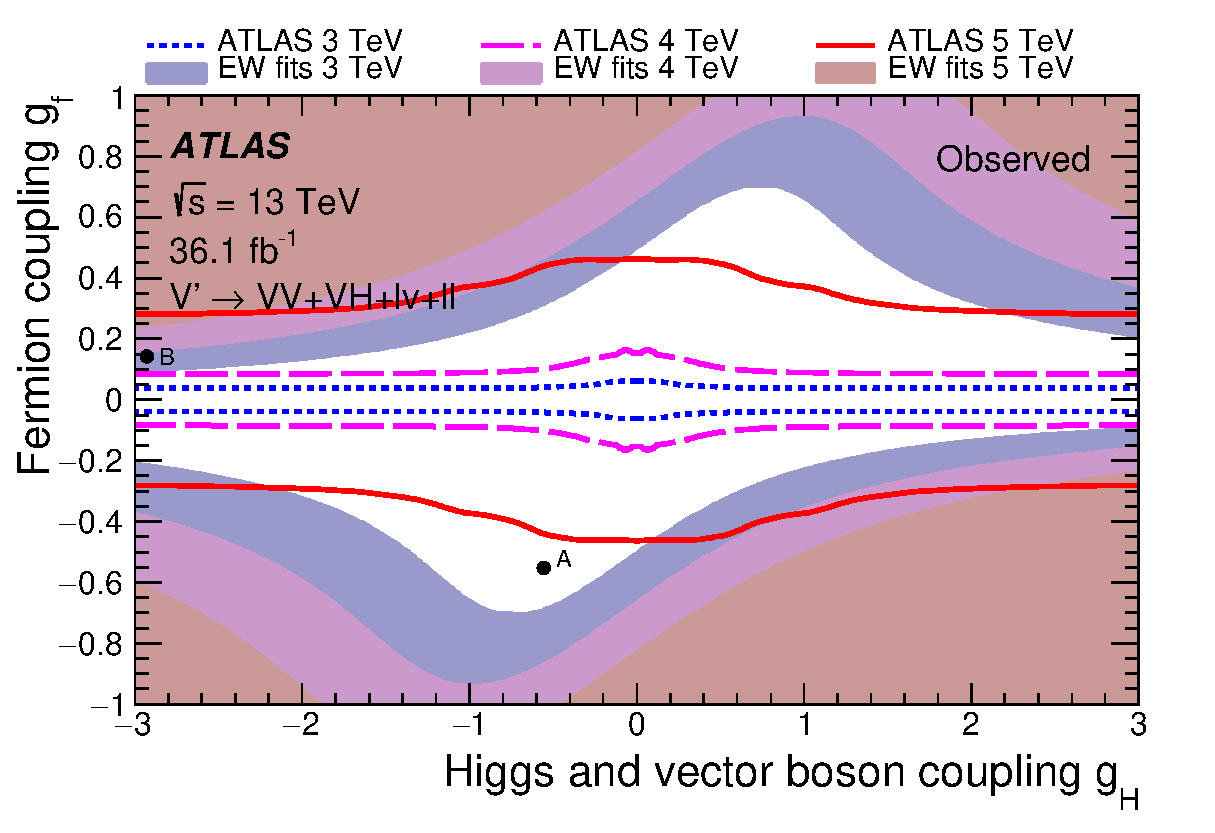
\includegraphics[width=0.5\textwidth]{Chapter4/Coupling_hf_all.eps}}
	\subfloat[]{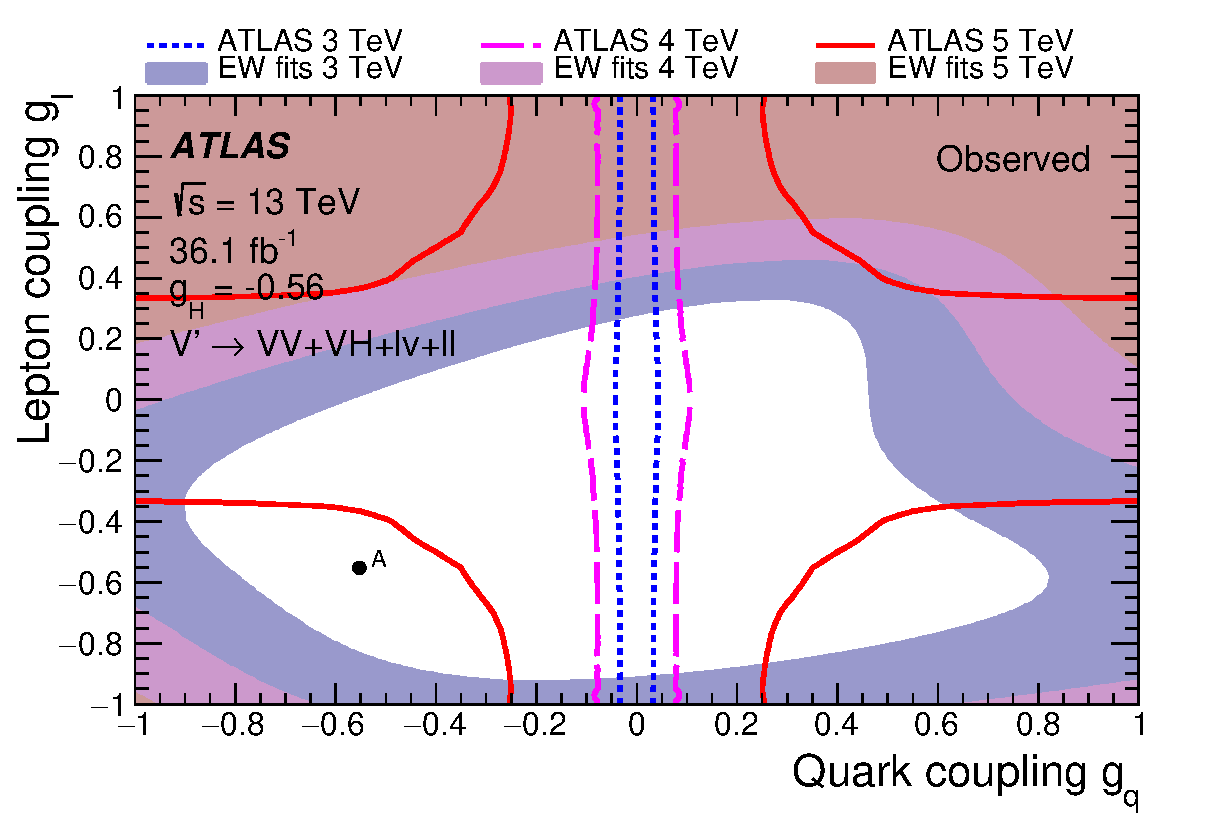
\includegraphics[width=0.5\textwidth]{Chapter4/Coupling_lg_all.eps}}
	\caption{The limits on coupling strength from the full combination with (a) {$g_H, g_f$} and (b) {$g_l, g_q$} planes }
	\label{Fig:limit_coupling}
\end{figure}
\noindent
\\
\\It could be seen that the combination of exotic particle searches has presented the exclusion that the electroweak measurements did not have the sensitivity to achieve. With the low mass HVT boson assumptions, both of the two benchmark models are also excluded by the coupling strength interpretation.
\section{Summary}
In the search for new particles with diboson resonance, the single final state of $WV\to\ell\nu qq$ is chosen to investigate two production modes, ggF/DY (indistinguishable) and VBF, along two jet topologies. The background estimation was performed with the Monte Carlo simulation for the Standard Model process like W+jets and $t\bar{t}$ interactions and the Fake Factor method for the multijet events. After the comparison between background estimation and data with a statistic interpretation, the discovery significance did not confirm the existence of any unknown particle. Therefore, the limits are set via the asymptotic method on the particle mass based the present analysis sensitivity. 
\\
\\For the further enhancement on the sensitivity to new physics, the $\ell\nu qq$ result was combined with the other diboson and dilepton final states. However, there is still no evident existence of the new particles. The limits on the particle mass and their coupling to the SM particle are then set giving an improved constraint on the phase space for the new particle searches.  